\documentclass[dutch]{uhphyspaper} 
%%%%%%%%%%%%%%%%%%%%%%%%%%%%%%
%       START DOCUMENT       %
%%%%%%%%%%%%%%%%%%%%%%%%%%%%%%
\usepackage{lipsum} % For demo purposes, remove 
\usepackage{listings} % Provides \lstinline{} for demo, remove


% Titles
\title{Gravitationele Lensen}
\runningtitle{*Running title: \textit{Short title ($\mathit{< 50}$ characters inc. spaces, italic, leave empty if not needed)}}
\keywords{list at least five keywords, separated by commas}

% Course information
\bachyear{$\mathit{3^{e}}$}
\course{Bachelorproef}
\date{\today}

% Authors, supervisors, principle investigator (PI, promotor)
\author[1]{Yara Roelen}
\author[4$^{\dagger}$]{Jori Liesenborgs} % Promotor: Dagger here signifies that the PI is the main correspondent

% Author affiliations
\affil[1]{UHasselt, Agoralaan, 3590 Diepenbeek, Belgium}
\affil[2, 3]{Computational Sciences}
\affil[1,4$^{\dagger}$]{UHasselt, EDM, Agoralaan, 3590 Diepenbeek, Belgium} % Dagger here signifies that the PI is the main correspondent

% PI contact info, do not remove
\pitel{+32 (11) 11 11 11}
\pimail{PImail@uhasselt.be}


%%%%%%%%%%%%%%%%%%%%%%%%%%%%%%
%       START DOCUMENT       %
%%%%%%%%%%%%%%%%%%%%%%%%%%%%%%
\begin{document}
\maketitle\thispagestyle{fancy} % pagestyle ensures header is present

% Each section is placed in a separate file to better organise your text
% You can find these files in the Sections folder
\section*{ABSTRACT}
% Edit below
\textbf{Bij gravitationele lenzing kan het voorkomen dat een object afgebeeld wordt op meerdere beelden. Soms komt het voor dat een beeld achter de lens (een zware massa) staat. Dan kan nuttige informatie over de massaverdeling van de lens niet gevonden worden.\\ \\
Om toch informatie te kunnen bekomen over de zware massa moet het beeld dat achter de zware massa staat gevonden worden. Dat wordt gedaan op drie verschillende manieren, allen gebaseerd op de stelling van Bayes: de kansdichtheid, het Metropolis algoritme en de emcee library. Alle drie de methodes geven gelijkende resultaten. \\ \\
Eerst werd het Metropolis algoritme uitgetest. Dat werkt goed vanaf een voldoende groot aantal samples. Nadien werd met de kansdichtheid en het Metropolis algoritme informatie over een signaal met achtergrondruis verzameld. Ook dit werkte goed. Bij het signaal en de ruis waren er twee onbekende parameters. Dit werd uitgebreid naar zes parameters, de parameters van de zware massa (een sersic). Ook het afschatten van alle parameters van een sersic is gelukt. \\ \\
Het is ook gelukt om de parameters van een systeem bestaande uit twee sersics af te schatten. Er werd een zware massa op een werkelijke achtergrond (gemodelleerd door NASA) geplaatst. Hier werd er opnieuw geprobeerd om de parameters van de zware massa zo goed mogelijk af te schatten, zodat de achtergrond zichtbaar wordt. Dit is niet volledig gelukt, doordat de achtergrond te ruisig was en er op die manier geen nauwkeurige afschatting van de parameters van de sersic gemaakt konden worden. In de toekomst zou voor dit probleem AI gebruikt kunnen worden.}
\newline
\rule[1.5ex]{\linewidth}{0.4pt}

\section{INTRODUCTION}
Gravitationele lensing is een effect dat optreedt wanneer licht afgebogen wordt door het gravitatieveld van massieve objecten, zoals sterrenstelsels of donkere materie \cite{informationesoorg-no-date}. De afbuiging van het licht kan zowel Newtoniaans als gravitationeel afgeleid worden. De Newtoniaanse afleiding voor een hyperbolische baan is te vinden in \cref{appendix: newton}. In tegenstelling tot klassieke lensing, waarbij één object wordt afgebeeld op één ander object, kan bij gravitationele lensing één object afgebeeld worden op meerdere objecten \cite{unknown-author-2022}. Dit wordt bepaald door de lensvergelijking. De afleiding van de lensvergelijking in 1D is te vinden in \cref{appendix:lensvergelijking}.\\ \\
Door de afbuiging van het licht als gevolg van het zwaartekrachtveld van een zware massa (denk aan een sterrenstelsel, donkere materie ...) 
worden de objecten niet waargenomen op de plaats waar ze effectief staan \cite{lea-2023}. Vanuit de plaats waarop het object waargenomen wordt, kan de effectieve positie bepaald worden. Stel nu dat het object afgebeeld wordt op meerdere deelobjecten, dan moeten alle deelobjecten teruggerekend worden. Dit kan op een zeer analoge manier als bij één object. \\ \\
Soms kan het voorkomen dat een object afgebeeld wordt achter de zware massa zelf. Dan is de kans dat het beeld niet gevonden wordt reëel. Het is echter wel noodzakelijk om alle beelden te hebben om de effectieve positie van het object te kunnen achterhalen. Het doel van deze bachelorproef is het wegwerken van de zware massa op de voorgrond, om het beeld dat op de achtergrond staat waar te kunnen nemen. Het vinden van het beeld dat op de achtergrond staat kan ook heel nuttig zijn om informatie te bekomen over de massaverdeling van de zware massa. Zeker als onze zware massa donkere materie is, kan het interessant zijn om meer te weten te komen over de massaverdeling ervan. \\ \\
Er bestaan al een heel aantal manieren waarop dit gedaan kan worden. Voorbeelden hiervan zijn IMFIT \cite{chen-2020}, \cite{erwin-2015} en GALFIT \cite{peng-2010}, \cite{unknown-author-no-date-galfit}.
In deze bachelorproef wordt er gebruik gemaakt van Bayesiaanse statistiek en deep learning.




\section{THEORIE}
% Edit below
\subsection{De lensvergelijking}
    %\begin{align}
    %x \times x   &= (x \times x) + 0  &&\textit{ Neutr. El. }+\\
    %        &= (x \times x) + (x \times \neg x) && \textit{ %Compl. }\times \\
    %        &= x + (x \times \neg x) && \textit{ Distr. }+ \\
    %        &= x + 0 && \textit{ Compl. }\times\\
    %        &= x && \textit{ Neutr. El. }+
    %\end{align}
De werking van de lens kan benaderd worden als een geometrisch probleem in twee dimensies. De voorstelling van de werking van de lens is te zien in \cref{fig:lensvgl}
\begin{figure}[H]
    \centering
    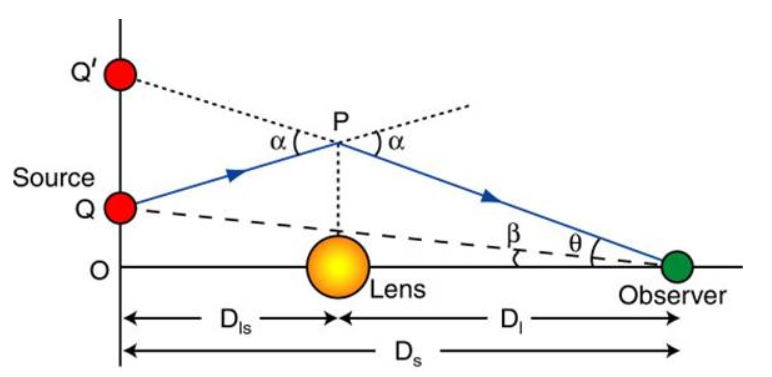
\includegraphics[scale=0.5]{Figures/Lensvergelijking.png}
    \caption{Schets van de werking van de lens in twee dimensies.}
    \label{fig:lensvgl}
\end{figure}\mbox{}
Om de lensvergelijking af te leiden wordt er gezocht naar de afstanden $OQ$, $OQ'$ en $QQ'$. Er wordt steeds aangenomen dat de hoeken klein zijn. Uit de figuur volgt er dat
$$tan(\beta) = \frac{|OQ|}{D_{s}}$$
$$|OQ| = D_{s}tan(\beta)$$
Doordat de hoeken klein zijn kunnen we Taylor rond $\beta=0$ toepassen. Er word dan gevonden dat
\begin{equation}
  |OQ| = D_{s}\beta  
  \label{for:OQ}
\end{equation}
Analoog voor $|OQ'|$ geldt er
\begin{equation}
   |OQ'| = D_{s}\theta 
   \label{for:OQ'}
\end{equation}
Om de afstand $|QQ'|$ te bepalen wordt er gewerkt in de driehoek $\Delta PQQ'$. Een close-up van de driehoek is te zien in \cref{fig:driehoek}.
\begin{figure}[h]
    \centering
    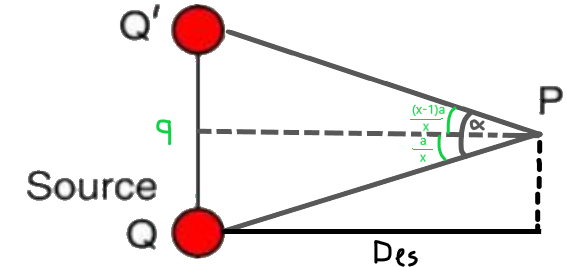
\includegraphics[scale=0.45]{Figures/driehoek.png}
    \caption{Close-up van de desbetreffende driehoek}
    \label{fig:driehoek}
\end{figure}
Er wordt opgemerkt dat $|QQ'| = |Qq|+|qQ'|$. Die twee afstanden zijn makkelijk te vinden uit de tangens. De hoek $\alpha$ wordt gesplitst in twee hoeken (die optellen tot $\alpha$). Zo wordt een rechthoekige driehoek verkregen. De eerste hoek is dan $\frac{\alpha}{x}$. De tweede hoek is gegeven door $\frac{(x-1)\alpha}{x}$. Zo zijn de twee afstanden gegeven door
$$tan(\frac{\alpha}{x})=\frac{|Qq|}{D_{ls}}$$
$$|Qq|=tan(\frac{\alpha}{x})D_{ls}$$
Analoog wordt er gevonden
$$tan(\frac{(x-1)\alpha}{x})=\frac{|qQ'|}{D_{ls}}$$
$$|qQ'|=tan(\frac{(x-1)\alpha}{x})D_{ls}$$
De som is dan gegeven door
$$|QQ'|=D_{ls}(tan(\frac{\alpha}{x})+tan(\frac{(x-1)\alpha}{x}))$$
Doordat de hoek $\alpha$ klein is kan er Taylor toegepast worden op de tangens, rond 0. Dan wordt er gevonden dat
\begin{align}
    |QQ'| &=D_{ls}(\frac{\alpha}{x}+\frac{x\alpha}{x}-\frac{\alpha}{x}) \nonumber\\
    &=D_{ls}\alpha
    \label{for:QQ'}
\end{align}
Nu de afstanden $|OQ|, |OQ'|$ en $|QQ'|$ gekend zijn (zie \cref{for:OQ}, \cref{for:OQ'} en \cref{for:QQ'}), kan de lensvergelijking gevonden worden. Het is eenvoudig in te zien dat $|OQ'|=|OQ|+|QQ'|$. Daaruit volgt
\begin{align}
    D_{s}\theta &=D_{s}\beta + D_{ls}\alpha \nonumber\\
    \theta &= \beta + \frac{D_{ls}}{D_{s}}\alpha \nonumber\\
    \beta &= \theta - \frac{D_{ls}}{D_{s}}\alpha
    \label{for: lensvgl}
\end{align}
\cref{for: lensvgl} wordt de lensvergelijking genoemd.
\subsection{Newtoniaanse bepaling afbuighoek als gevolg van een gravitationeel veld}
Er wordt vertrokken vanuit de bewegingsvergelijkingen voor een deeltje in een potentiaal, gecreëerd door het zwaartekrachtveld. Er wordt aangetoond dat de oplossingen van de bewegingsvergelijking kegelsneden (cirkel, ellips, hyperbool, parabool) als oplossing heeft.
\subsubsection{De baan van een deeltje in een zwaartekrachtveld zijn kegelsneden}
Voor gravitatie wordt de potentiële energie gegeven door
$$V(r)=-\frac{GmM}{r}$$
De effectieve potentiële energie is gegeven door
$$V_{eff}(r)=-\frac{k}{r}+\frac{l^{2}}{2\mu r^{2}}$$
Hierin is $k=GmM$.\\
De bewegingsvergelijking wordt dan gegeven door
$$\mu\ddot{r}=\frac{l^{2}}{\mu r^{3}}-\frac{k}{r^{2}}$$
Deze vergelijking is niet lineair. We voeren een nieuwe variabele in. Stel $u=\frac{1}{r}$ en $t=\phi$. We weten al dat
$$\mu r^{2}\dot{\phi}=l;\ \ \ \ \ \mu r^{2}d\phi=ldt;\ \ \ \ \ dt=\frac{\mu}{lu^{2}}d\phi$$
Dan geldt er dat
\begin{align}
\dot{r}&=\frac{d}{dt}r=\frac{d}{dt}(\frac{1}{u}) \nonumber \\
&=-\frac{1}{u^{2}}\frac{du}{dt} \nonumber \\
&=-\frac{1}{u^{2}}\frac{du}{d\phi}\frac{d\phi}{dt} \nonumber \\
&=-\frac{1}{u{2}}\frac{lu^{2}}{\mu}\frac{du}{d\phi} \nonumber \\
&=-\frac{l}{\mu}\frac{du}{d\phi} \nonumber 
\end{align}
De 2de afgeleide is gegeven door
\begin{align}
\ddot{r}&=\frac{d}{dt}[-\frac{l}{\mu}\frac{du}{dt}] \nonumber \\
&=-\frac{l}{\mu}\frac{d}{d\phi}(\frac{du}{d\phi})\frac{d\phi}{dt} \nonumber \\
&=-\frac{l}{\mu}\frac{lu^{2}}{\mu}\frac{d^{2}u}{d\phi^{2}} \nonumber 
\end{align}
Dan krijgen we als differentiaalvergelijking van de baan dat
$$\frac{d^{2}u}{d\phi^{2}}+u=\frac{k\mu}{l^{2}}$$
De oplossing van deze differentiaalvergelijking is gegeven door
$$u(\phi)=\frac{\mu k}{l^{2}}+Acos(\phi)$$
We gaan nu overgaan op Cartesische coördinaten. Stel $p=\frac{l^{2}}{\mu k}$ en stel $\epsilon=pA\geq0$. Dan geldt er
$$pu=1+\epsilon cos(\phi)$$
$$p=r+r\epsilon cos(\phi)$$
$$(p-\epsilon x)^{2}=x^{2}+y^{2}$$
De energie is gegeven door
$$E=\frac{1}{2}\mu(\dot{r}^{2}+r^{2}\dot{\phi}^{2})-\frac{k}{r}$$
$$=\frac{\mu k^{2}}{2l^{2}}(\epsilon^{2}-1)$$
Merk op dat de energie afhankelijk is van $\epsilon$. 
\begin{itemize}
\item  $\epsilon=0$: we hebben een minimum van de energie. Er geldt
$$x^{2}+y^{2}=p^{2}$$
Dit is exact gelijk aan de vergelijking van een cirkel met als straal p. Deze straal is exact gelijk aan het minimum van $V_{eff}$. 
\item $\epsilon=1$, dan is de energie gelijk aan 0. De baan is dan gegeven door
$$p{2}+x^{2}-2px=x^{2}+y^{2}$$
$$2px=p^{2}-y^{2}$$
$$x(y)=\frac{p^{2}-y^{2}}{2p}$$
Dit is de baan van een parabool
\item $0<\epsilon<1$, dit komt overeen met een energie die kleiner is dan 0. De baan is dan gegeven door
$$p^{2}+\epsilon^{2}x^{2}-2\epsilon px-x^{2}-y^{2}=0$$
$$(1-\epsilon^{2})x^{2}+2\epsilon px+y^{2}-p^{2}=0$$
$$(1-\epsilon^{2})(x^{2}+\frac{2\epsilon px}{(1-\epsilon^{2})}+\frac{\epsilon^{2}p^{2}}{(1-\epsilon^{2})^{2}}-\frac{\epsilon^{2}p^{2}}{(1-\epsilon^{2})^{2}})+y^{2}-p^{2}=0$$
$$(1-\epsilon^{2}))(x+\frac{\epsilon p}{(1-\epsilon^{2})})^{2}+y^{2}-\frac{\epsilon^{2}p^{2}}{(1-\epsilon^{2})}-p^{2}=0$$
$$(1-\epsilon^{2})(x+\frac{\epsilon p}{(1-\epsilon^{2})})^{2}+y^{2}=\frac{p^{2}}{(1-\epsilon^{2})}$$
Dit kunnen we ook nog schrijven als
$$\frac{(x-x_{c})^{2}}{a^{2}}+\frac{y^{2}}{b^{2}}=1$$
Met: \\
$x_{c}=\frac{-\epsilon p}{1-\epsilon^{2}}$ \\
$p=\frac{l^{2}}{\mu k}$\\
$\epsilon = pA$\\
$a=\frac{p}{1-\epsilon^{2}}$\\
$b=\frac{p}{\sqrt{1-\epsilon^{2}}}$\\
Dit komt overeen met de baan van een ellips
\item $\epsilon > 0$, dit komt overeen met een energie die groter is dan 0. 
$$\frac{(x-x_{c})^{2}}{a^{2}}-\frac{y^{2}}{b^{2}}=1$$
Dit is de baan van een hyperbool
\end{itemize}
\subsubsection{De bijhorende afbuighoek voor een hyperbolische baan}
De kinetische energie van het deeltje in de potentiaal (per eenheidsmassa) is gegeven door 
\begin{equation}
    E=\frac{1}{2}mv^{2}
    \label{for:energie}
\end{equation}
Het draaimoment per eenheidsmassa is gegeven door
\begin{equation}
    L=rv
    \label{for:draaimoment}
\end{equation}
Deze twee grootheden kunnen ook geschreven worden in termen van de lange en korte as van de kegelsneden:
\begin{equation}
    E = \frac{GM}{2a}
    \label{for:E}
\end{equation}
\begin{equation}
    L^2 = \frac{GMb^{2}}{a}
    \label{for:L2}
\end{equation}
De halve hoek van de hyperbolische baan is dan gegeven door 
\begin{equation}
    tan(\beta) = \frac{b}{a}
    \label{for: hoek}
\end{equation}
We gaan \cref{for: hoek} herschrijven in termen van L (\cref{for:L2}) en E (\cref{for:E}).
Merk op dat
$$E\cdot L^{2}=\frac{G^{2}M^{2}b^{2}}{2a^{2}}$$
$$\frac{2E\cdot L^{2}}{G^{2}M^{2}}=\frac{b^{2}}{a^{2}}$$
$$\frac{\sqrt{2E}L}{GM}=\frac{b}{a}$$
Invullen van \cref{for:energie} en \cref{for:draaimoment} geeft
\begin{align}
    \frac{b}{a}&=\frac{\sqrt{2\cdot\frac{1}{2}v^{2}}rv}{GM} \nonumber \\
    &= \frac{rv^{2}}{GM} \nonumber \\
    tan(\beta) &=\frac{rv^{2}}{GM} 
    \label{for:tangens}
\end{align}
Voor de afbuighoek geldt er dan:
$$\theta = \pi - 2\beta$$
Omvormen naar $\beta$ geeft
$$\beta = \frac{\pi}{2}-\frac{\theta}{2}$$
De tangens nemen
\begin{equation}
    tan(\beta) = tan(\frac{\pi}{2}-\frac{\theta}{2})
    \label{for:tan}
\end{equation}
We herschrijven de laatste tangens:
\begin{align}
    tan(\frac{\pi}{2}-\frac{\theta}{2})&=\frac{sin(\frac{\pi}{2}-\frac{\theta}{2})}{cos(\frac{\pi}{2}-\frac{\theta}{2})}\nonumber\\
    &= \frac{cos(\frac{\theta}{2}}{sin(\frac{\theta}{2}}\nonumber \\
    & = cot(\frac{\theta}{2})
    \label{for:cot}
\end{align}
Invullen van \cref{for:cot} in \cref{for:tan} geeft
\begin{equation}
    tan(\beta) = \frac{1}{tan(\frac{\beta}{2})}
    \label{for:afbuighoek}
\end{equation}
Invullen van \cref{for:tangens} en Taylor toepassen voor kleine $\theta$
$$\frac{1}{tan(\frac{\theta}{2})} = \frac{rv^{2}}{GM}$$
$$\frac{1}{\frac{\theta}{2}}=\frac{rv^{2}}{GM}$$
$$\frac{\theta}{2} = \frac{GM}{rv^{2}}$$
$$\theta = \frac{2GM}{rv^{2}}$$
Als de afbuiging van licht beschouwd wordt is de snelheid gegeven door de snelheid van het licht. Dan is de afbuighoek gegeven door \cref{for: afbuighoek}.
\begin{equation}
    \theta = \frac{2GM}{rc^{2}}
    \label{for: afbuighoek}
\end{equation}
Dit was nu de afleiding voor de hyperbool. 
\\ ???? KAN DAT ???? \\
Als het foton geen hyperbolische baan volgt, dan komt het vast te zitten. Uit de 2de wet van Kepler volgt ook dat gelijke oppervlakken in gelijke tijd beschreven worden. Daaruit volgt dan dat de snelheid van het deeltje afhankelijk is van de kromming van de baan. En dat is een probleem, want onze snelheid is de lichtsnelheid, en die kan niet groter worden. Een hyperbolische baan (of parabolisch, dat is gewoon een speciaal geval van de hyperbool) is dus de enige optie.
Analoog kan hetzelfde gedaan worden voor de ellips en parabool. Het enige dat verandert is de energie.\\
Voor de ellips geldt:
$$E=-\frac{GM}{2a}$$
Voor de parabool geldt:
$$E=0$$


 % May be removed if unnecessary
\section{EXPERIMENTAL PROCEDURES}
Het onderzoek werd gedaan met behulp van de programmeertaal Python (versie 3.12). Er werd gebruik gemaakt van de standaard library \cite{unknown-author-no-date-python}. Verder werden volgende library's nog gedownload:
\begin{itemize}
    \item numpy (versie 1.26.4)
    \item matplotlib.pyplot (versie 3.8.3)
    \item emcee (versie 3.1.4)
    \item scipy (versie 1.12.0)
\end{itemize}
 % May be removed if unnecessary
\section{RESULTS}
\subsection{Visualisatie van het Metropolis algoritme}
In het Metropolis algoritme worden samples genomen van een gewenste kansdichtheid. Er wordt steeds begonnen vanaf een gekozen positie. In het begin kan er niet veel afgeweken worden van die positie doordat er steeds maar kleine stapjes gezet worden. De eerste data die gegenereerd wordt komt dan ook nog niet goed overeen met de gewenste kansverdeling. Daarom worden steeds de eerste gegenereerde datapunten weggegooid. \\ \\
Om dit te laten zien werd een klein programma geschreven dat probeert om een kansverdeling na te maken. Om de 90 stappen wordt de stand van zaken afgebeeld op een figuur waarop zowel de huidige kansverdeling als de gewilde kansverdeling te zien is. Deze visualisatie is te zien in \cref{fig: visualisatie_metropolis}.
\begin{figure}
    \centering
    \begin{minipage}{0.49\linewidth}
        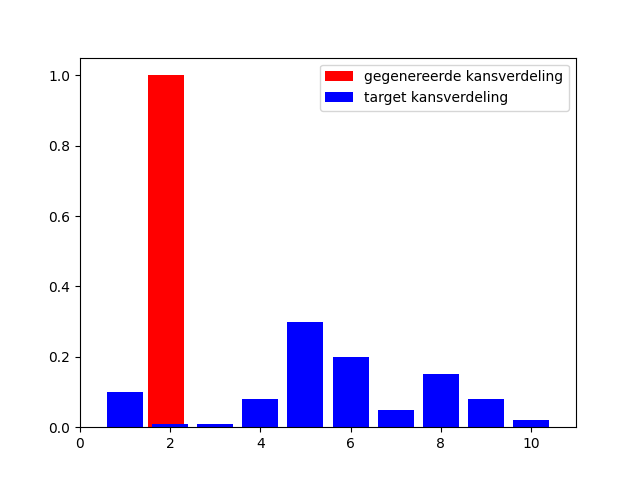
\includegraphics[width=\linewidth]{Figures/goede_visualisatie_legende/visualisatie_0.png} 
        \subcaption{na stap 0}
    \end{minipage}
    \hfill
    \begin{minipage}{0.49\linewidth}
        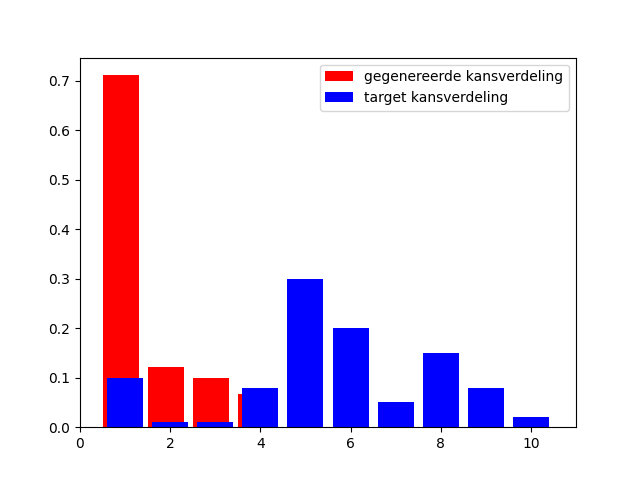
\includegraphics[width=\linewidth]{Figures/goede_visualisatie_legende/visualisatie_90.png}
        \subcaption{na stap 90}
    \end{minipage}
    \begin{minipage}{0.49\linewidth}
        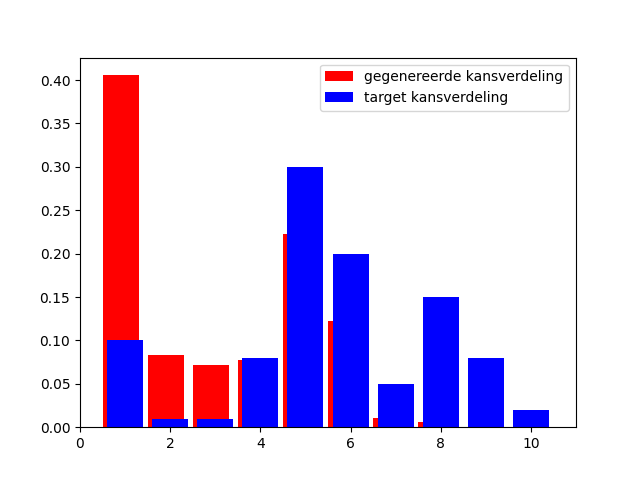
\includegraphics[width=\linewidth]{Figures/goede_visualisatie_legende/visualisatie_180.png} 
        \subcaption{na stap 180}
    \end{minipage}
    \hfill
    \begin{minipage}{0.49\linewidth}
        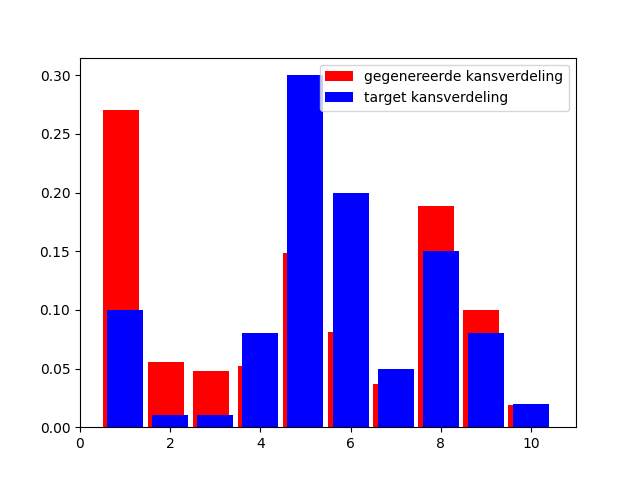
\includegraphics[width=\linewidth]{Figures/goede_visualisatie_legende/visualisatie_270.png}
        \subcaption{na stap 270}
    \end{minipage}
    \begin{minipage}{0.49\linewidth}
        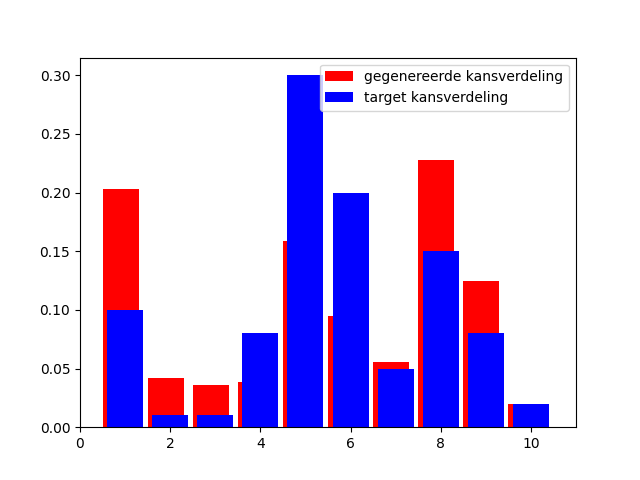
\includegraphics[width=\linewidth]{Figures/goede_visualisatie_legende/visualisatie_360.png} 
        \subcaption{na stap 360}
    \end{minipage}
    \hfill
    \begin{minipage}{0.49\linewidth}
        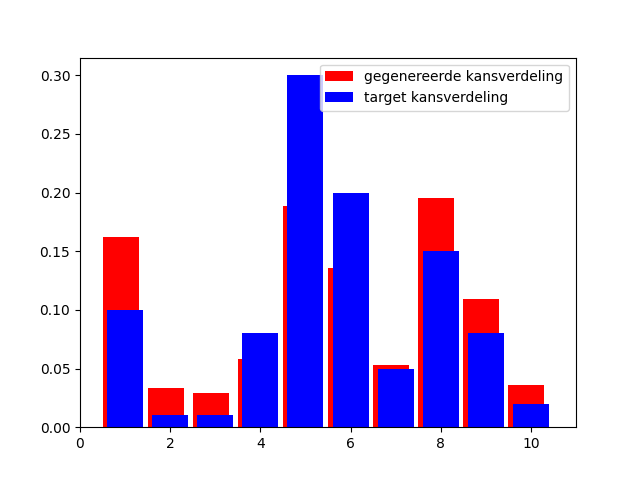
\includegraphics[width=\linewidth]{Figures/goede_visualisatie_legende/visualisatie_450.png}
        \subcaption{na stap 450}
    \end{minipage}
    \begin{minipage}{0.49\linewidth}
        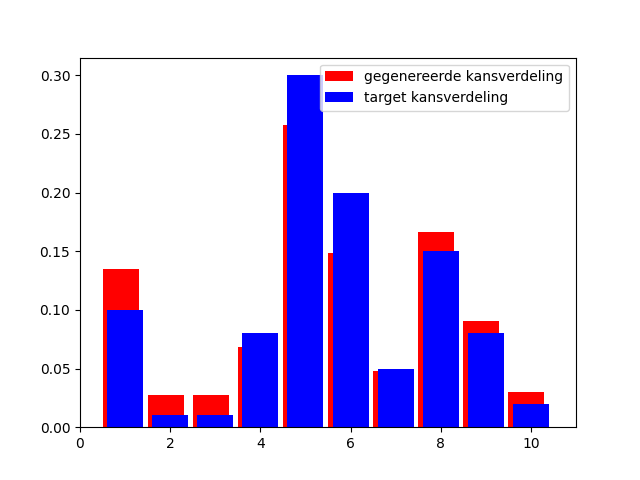
\includegraphics[width=\linewidth]{Figures/goede_visualisatie_legende/visualisatie_540.png} 
        \subcaption{na stap 540}
    \end{minipage}
    \hfill
    \begin{minipage}{0.49\linewidth}
        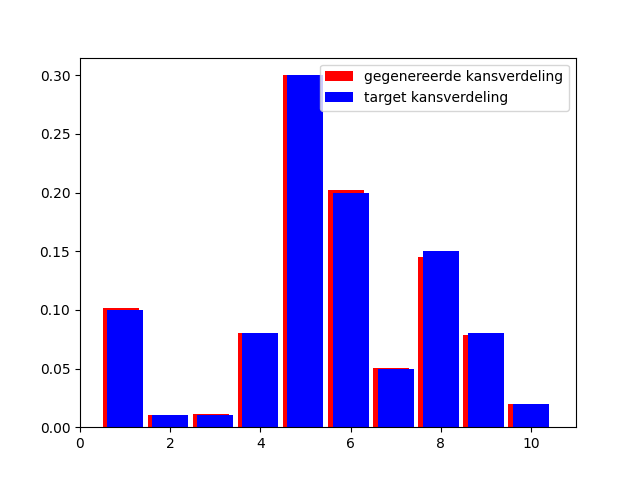
\includegraphics[width=\linewidth]{Figures/goede_visualisatie_legende/visualisatie_99999.png}
        \subcaption{na stap 100\_000}
    \end{minipage}
\caption{Visualisatie van het proces waarin toegewerkt wordt naar de gewenste kansverdeling. Op de bovenstaande figuren is de stand van zaken te zien na een vermeld aantal stappen. Het blauwe histogram is de target kansverdeling, het rode histogram is de huidige gesampelde kansverdeling.}
\label{fig: visualisatie_metropolis}
\end{figure}
Zoals te zien in de visualisatie (\cref{fig: visualisatie_metropolis}) heeft het algoritme wat tijd nodig om tot zijn target kansverdeling te komen. Na 90 stappen wordt de target kansverdeling nog niet benaderd, na 100\_000 stappen wordt bijna exact dezelfde kansverdeling als de target kansverdeling gevonden. Doordat die tijd nodig is om naar de target kansverdeling te gaan, heeft het pas zin om samples te halen uit de gewenste kansverdeling vanaf het moment dat de target benadert wordt. Om die reden worden heel vaak de eerste samples weggegooid. Zo start de sampeling pas vanaf het moment dat de target kansverdeling bij benadering bereikt is. Het exacte punt waarop de kansverdeling goed genoeg benadert wordt, is niet gekend.
\subsection{Signaal en achtergrondruis: stelling van Bayes en het Metropolis algoritme}
Voor er gestart werd met het schatten van de parameters van het sterrenstelsel en het achtergrondbeeldje, werd er gestart met het afschatten van een amplitude van een signaal in de aanwezigheid van achtergrondruis \cite{sivia-2006}. Dit werd gedaan gebruikmakende van de stelling van Bayes en later ook gebruikmakende van het Metropolis algoritme en de emcee library. Van de piek van het signaal en de achtergrond werd een 2D histogram gemaakt. De waarden werden ook gemarginaliseerd zodat ook het signaal en de achtergrond apart geplot konden worden. Ook werden op verschillende meetpunten $x$ het aantal tellingen bepaald. De figuren voor 1000 metingen en 25 databins, gebruikend makende van de stelling van Bayes zijn te vinden in \cref{fig:AB-bayes}. 
\begin{figure}
    \centering
    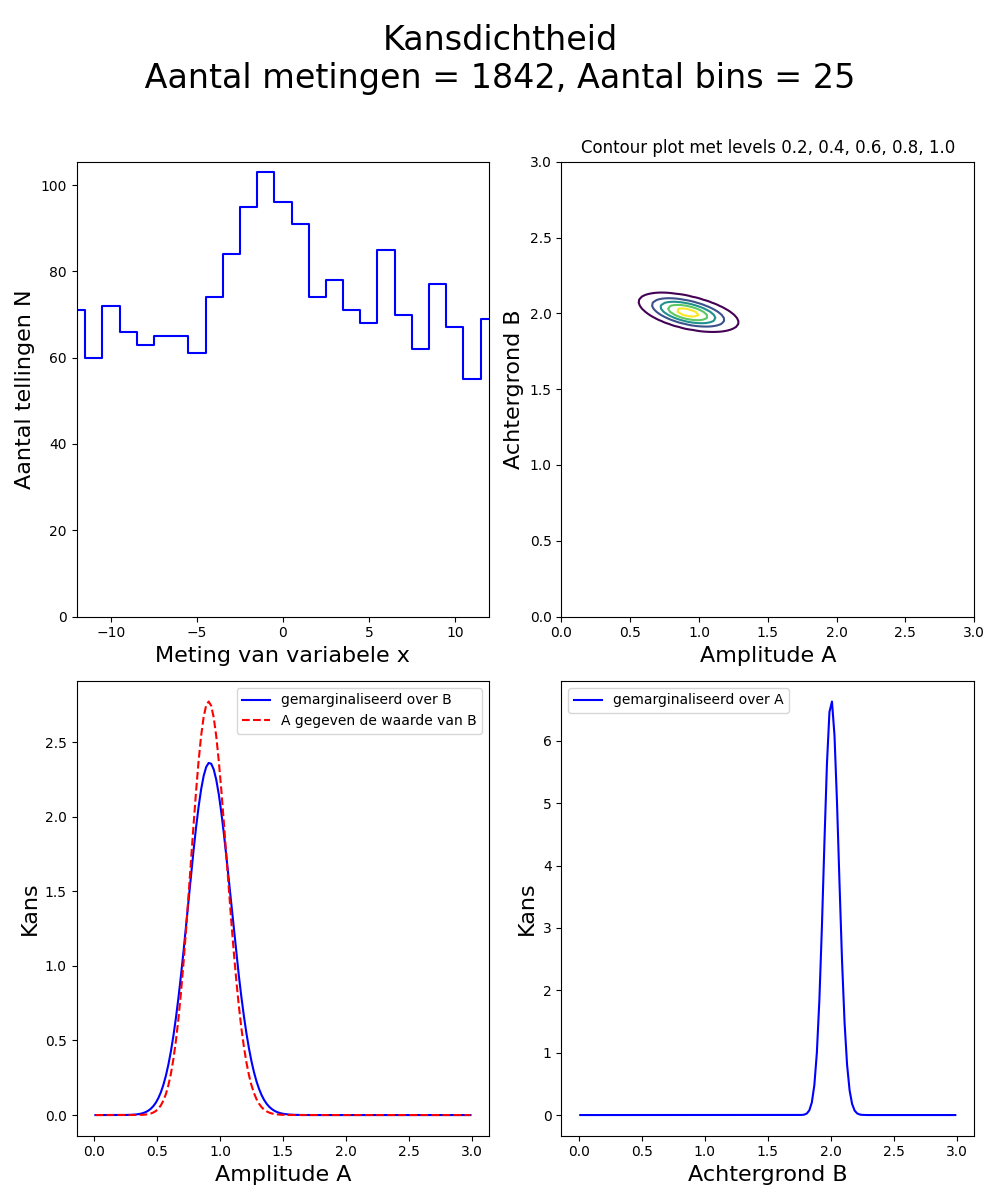
\includegraphics[width=0.45\textwidth]{Figures/figurenset1.png}
    \caption{\\Afbeelding 1: het aantal tellingen per datapunt x\\
    Afbeelding 2: 2D histogram van het signaal en de achtergrond \\
    Afbeelding 3: de amplitude van de piek, gemarginaliseerd over de achtergrond\\
    Afbeelding 4: de achtergrond, gemarginaliseerd over de amplitude van het signaal}
    \label{fig:AB-bayes}
\end{figure}\mbox{}
Nadien werd exact hetzelfde gedaan gebruikmakende van het Metropolis algoritme. Opnieuw werden dezelfde figuren gegenereerd. De figuren voor 1\_000\_000 metingen, waarvan er 60\_000 verwaarloosd zijn gebruikmakende van het Metropolis algoritme zijn te vinden in \cref{fig:AB-metropolis}.
\begin{figure}
    \centering
    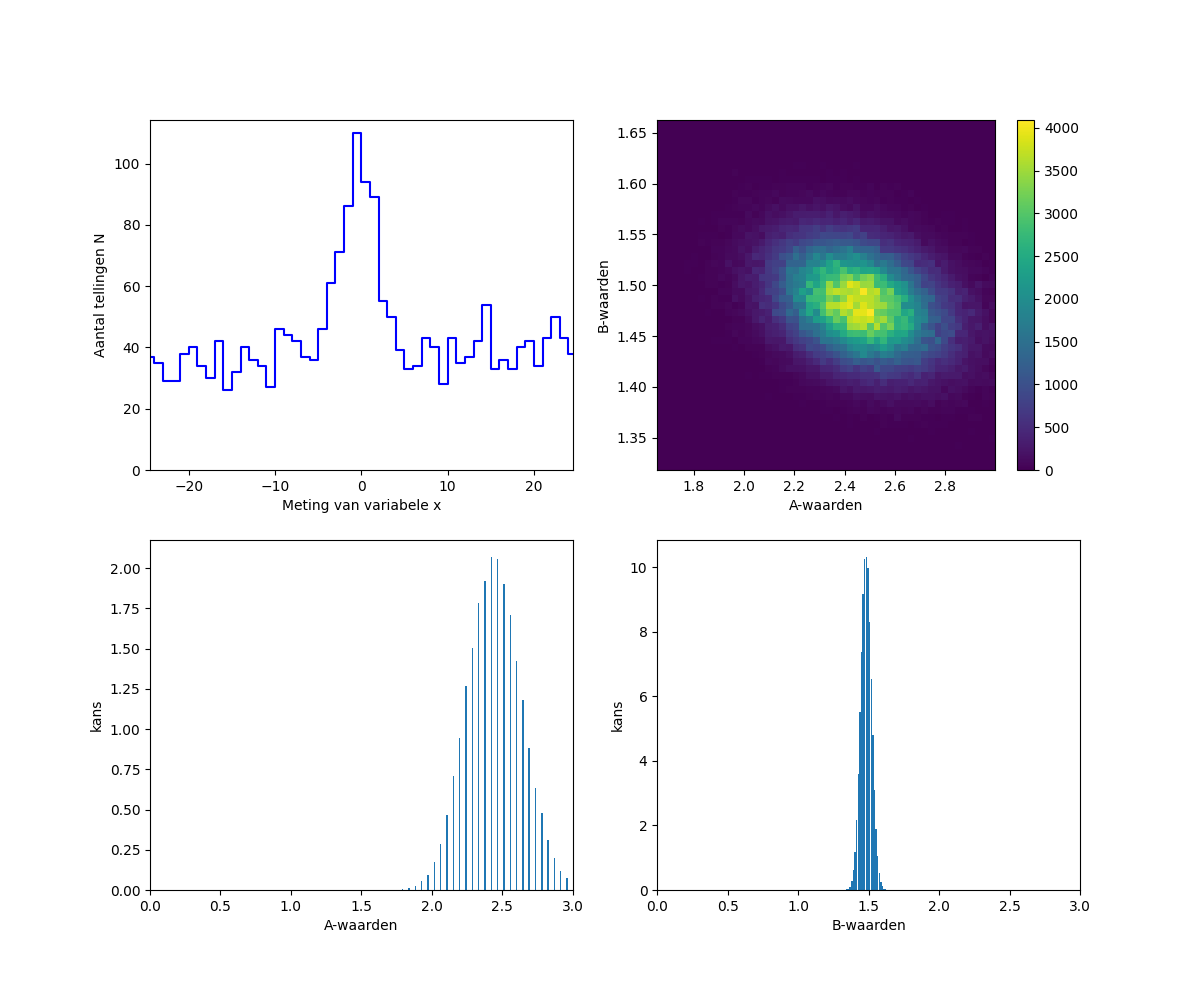
\includegraphics[width=0.95\linewidth]{Figures/signaal_AB_samples_1000000.png}
    \caption{\\Afbeelding 1: het aantal tellingen per datapunt x\\
    Afbeelding 2: 2D histogram van het signaal en de achtergrond \\
    Afbeelding 3: de amplitude van de piek, gemarginaliseerd over de achtergrond\\
    Afbeelding 4: de achtergrond, gemarginaliseerd over de amplitude van het signaal}
    \label{fig:AB-metropolis}
\end{figure}
Er wordt opgemerkt dat dit nagenoeg exact overeenkomt met de methode gebruikmakend van de stelling van Bayes. \\ \\Een laatste manier waarop samples verzameld kunnen wprden is door gebruik te maken van de emcee library. Deze library maakt gebruik van walkers. Een walker kan gezien worden als een enkel metropolis algoritme. Er wordt gestart op een beginpositie en wordt toegewerkt naar een target kansverdeling. Door gebruik te maken van meerdere walkers worden verschillende versies van de target kansverdeling gegenereerd. Door daar dan het gemiddelde over te nemen is de data stabieler. Exact hetzelfde voorbeeld werd nog eens gerunt door gebruik te maken van deze library. De grafieken kunnen gevonden worden in \cref{fig:AB_emcee}.
\begin{figure}
    \centering
    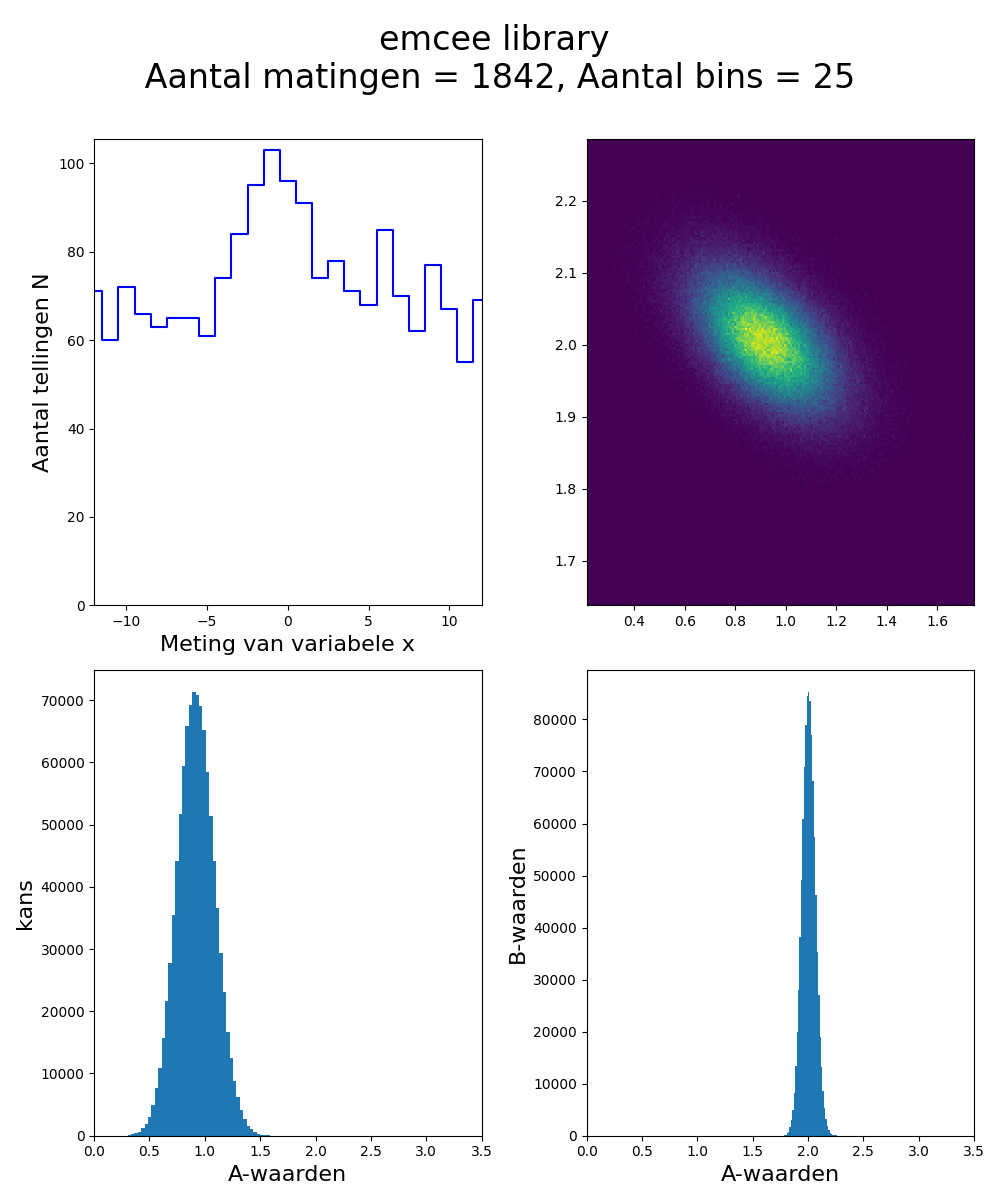
\includegraphics[width=0.95\linewidth]{Figures/emcee_hist_AB.png}
    \caption{\\Afbeelding 1: het aantal tellingen per datapunt x\\
    Afbeelding 2: 2D histogram van het signaal en de achtergrond \\
    Afbeelding 3: de amplitude van de piek, gemarginaliseerd over de achtergrond\\
    Afbeelding 4: de achtergrond, gemarginaliseerd over de amplitude van het signaal}
    \label{fig:AB_emcee}
\end{figure}
Ook hier worden dezelfde plots gevonden als in de voorgaande twee figuren (\cref{fig:AB-bayes} en \cref{fig:AB-metropolis}). Er kan geconcludererd wprden dat de data die geplot is in \cref{fig:AB_emcee} stabieler is. Het 2D-histogram is minder uitgesmeerd, en ook de gemarginaliseerde plots zijn scherper gepiekt en minder breed. Het uitmiddelen van de verschillende walkers leidt dus inderdaad tot betere data.\\ \\
Wat we er verder nog geconcludeerd kan worden is dat de drie manieren van werken equivalente resultaten opleveren. De gevonden data is in de drie gevallen ongeveer dezelfde. De pieken blijven op dezelfde plaats staan, de breedte van de pieken zelf kan wel veranderen afhankelijk van de methode.
\subsection{Afschatten van de parameters van een sersic}
Voor het modelleren van het lichtintensiteitsprofiel van het helder sterrenstelsel of het beeldje wordt er gewerkt met een 2D-sersic
\cite{unknown-author-no-date-sersic}
\cite{wikipedia-contributors-2024}. Die 2D-sersic beschrijft hoe de intensiteit van een sterrenstelsel varieert met de afstand ten opzichte van het centrum. Zo'n intensiteitsprofiel kan eenvoudig geplot worden met Python. Voor het plotten van een sersic moeten er zes parameters gekend zijn \cite{unknown-author-no-date-info-sersic};
\begin{enumerate}
    \item $x_{0}$: de $x$-positie van het middelpunt van het object
    \item $y_{0}$: de $y$-positie van het middelpunt van het object
    \item excentriciteit: een waarde tussen 0 en 1 waarbij 0 een cirkel is en 1 een parabool
    \item $r_{eff}$: de effectieve straal van het object, de straal waarbinnen de helft van het licht uitgestraald wordt \cite{wikipedia-contributors-2023-reff}
    \item amplitude: de helderheid van het object op een afstand $r_{eff}$ van het middelpunt
    \item $\theta$: de rotatiehoek van het object in radialen
\end{enumerate}
Stel al deze waarden zijn gekend, en zijn gelijk aan:
\begin{enumerate}
    \item $x_{0}$: 100
    \item $y_{0}$: 100
    \item excentriciteit: 0.3  
    \item $r_{eff}$: 25
    \item amplitude: 1
    \item $\theta$: $\frac{\pi}{4}$
\end{enumerate}
dan kan de 2D sersic getekend worden. Deze is te zien in \cref{fig: 2D_sersic}.
\begin{figure}
    \centering
    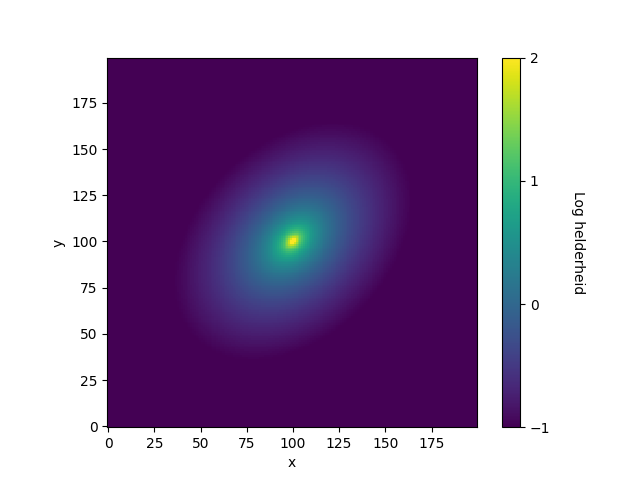
\includegraphics[width=0.95\linewidth]{Figures/figuur_2D_zonder_package_1_25_8_0.3_0.7853981633974483.png}
    \caption{2D sersic profiel}
    \label{fig: 2D_sersic}
\end{figure}
Wat nu geprobeerd wordt is de afschatting van de zes parameters, gegeven een object. Hiervoor wordt opnieuw gebruik gemaakt van het Metropolis algoritme of van de emcee library. 
\subsubsection{De afschatting van de parameters van een sersic}
Om te beginnen wordt er gebruik gemaakt van het Metropolis algoritme. Om de complexiteit gradueel op te voeren wordt eerst enkel $x_{0}$ afgeschat, waarna ook $y_{0}$, de excentriciteit ... volgen. Wanneer niet alle parameters geschat worden, worden de resterende parameters als gekend beschouwd. Er wordt een dataset gemaakt op basis van de echte waarden van het object. Om de situatie meer waarheidsgetrouw te maken, wordt op de dataset poissonruis toegevoegd. Uit de dataset waarop ruis toegevoegd is, wordt dan gesampled, in de hoop om de parameters van het object terug te vinden uit de dataset.
Er wordt gewerkt met volgende waarden voor de parameters:
\begin{enumerate}
    \item $x_{0}$: 16
    \item $y_{0}$: 16
    \item excentriciteit: 0.35 
    \item $r_{eff}$: 5
    \item amplitude: 50
    \item $\theta$: $\frac{\pi}{4}$
\end{enumerate}
De resultaten gebruikmakend van het Metropolis algoritme zijn te zien in \cref{appendix: opbouw}. Het eindresultaat, waarin alle zes de parameters afgeschat worden, is te zien in \cref{fig: 6 onbekenden}. Voor de afschatting van die zes parameters werden 9\_500\_000 samples gegenereerd waarvan er 1\_500\_000 weggegooid werden.
\begin{figure}
    \centering
    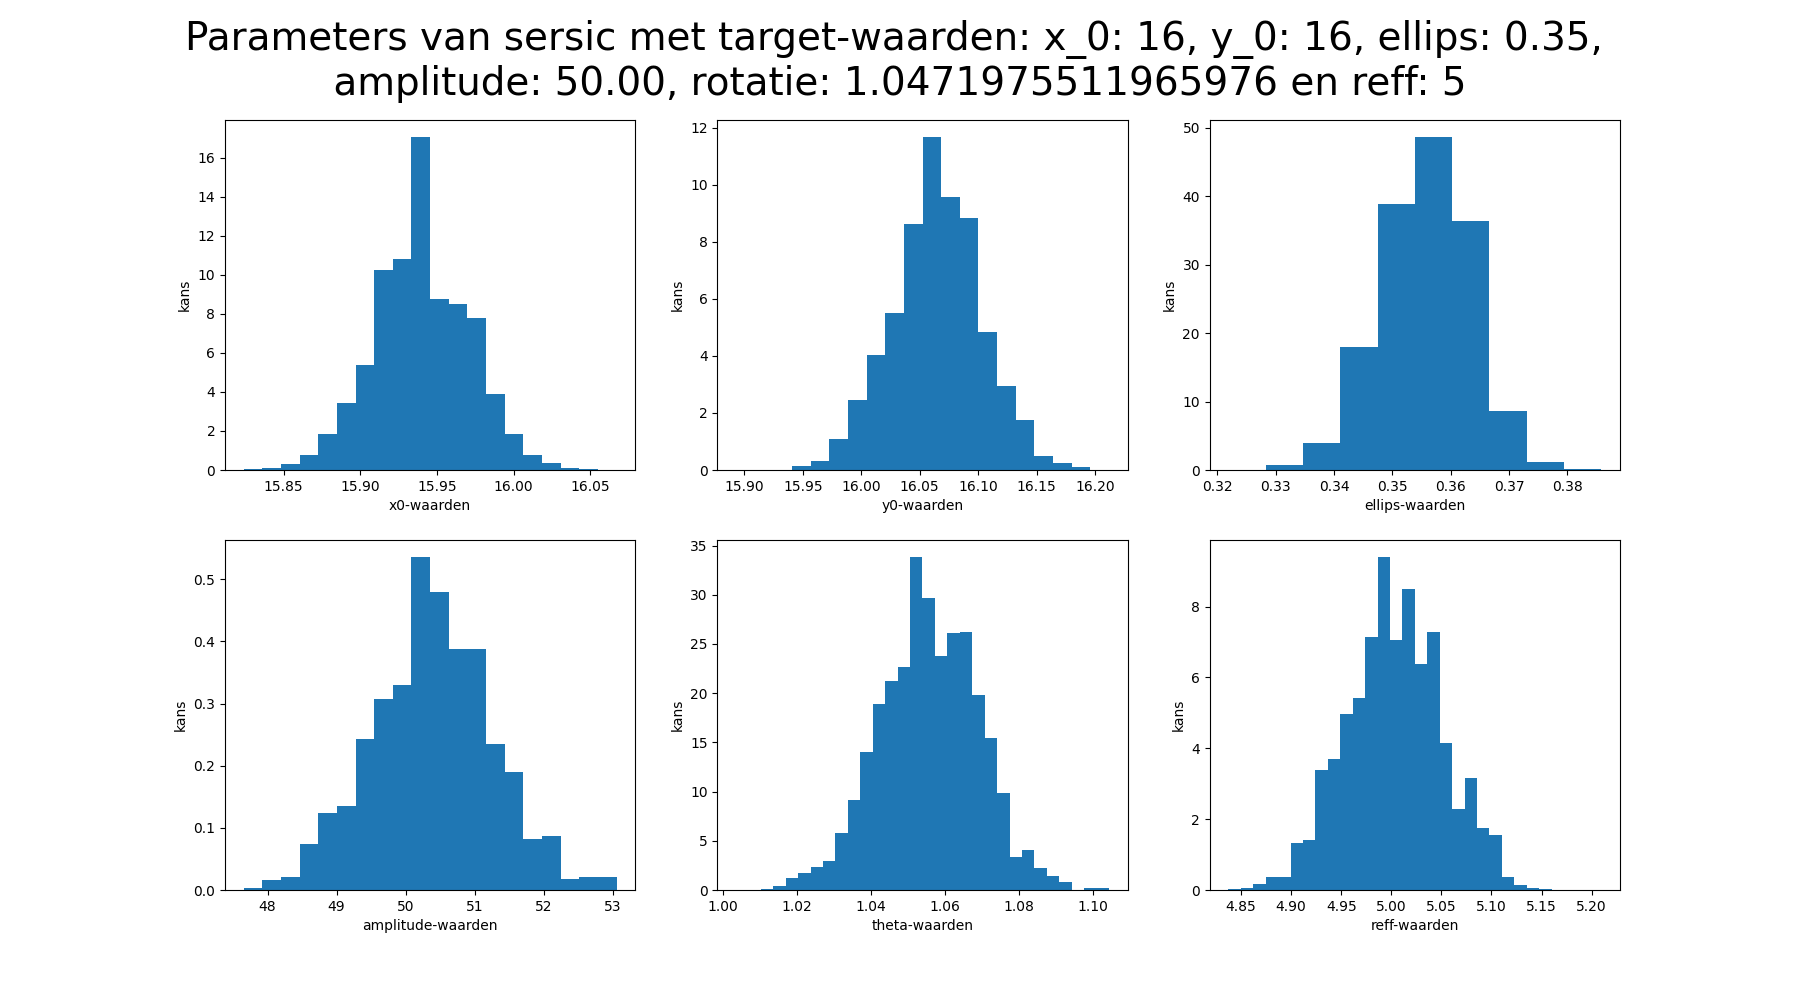
\includegraphics[width=0.95\linewidth]{Figures/sersic_parameters_metropolis_8500000_1500000_50_reff.png}
    \caption{Het resultaat van de afschatting van zes verschillende parameters van de sersic}
    \label{fig: 6 onbekenden}
\end{figure}
Zoals te zien in \cref{fig: 6 onbekenden} komen de pieken van afgeschatte parameters goed overeen met de effectieve waarden die gebruikt zijn om de dataset te generen. De afgeschatte parameters kunnen ook getoetst worden aan de bijhorende figuur van de sersic. Die figuur is te zien in \cref{fig: af te schatten sersic}. Op de figuur is inderdaad te zien dat de sersic ongeveer $14^{\circ}$ geroteerd is. Ook de x0 en y0 posities en de excentriciteit zijn te zien en komen inderdaad overeen met de waarden die afgeschat werden. 
\begin{figure}
    \centering
    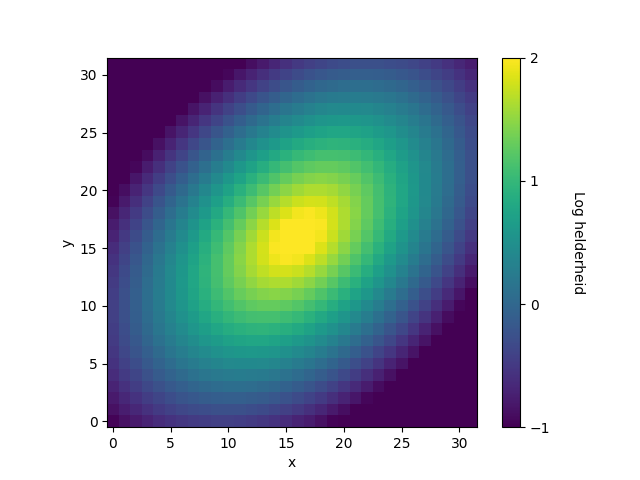
\includegraphics[width=0.95\linewidth]{Figures/figuur_2D_zonder_package_40_5_1_0.35_0.7853981633974483.png}
    \caption{Een 2D sersic gegenereerd volgens de paramters die gebruikt worden om de waarden van de sersic te zien in \cref{fig: 6 onbekenden} af te schatten.}
    \label{fig: af te schatten sersic}
\end{figure}\mbox{}\\
Hetzelfde kan nu gedaan worden met behulp van de emcee library. Hier worden alle zes de parameters meteen tegelijk afgeschat. Het resultaat van de afschatting met 100 walkers, 12000 stappen, waarvan er 2300 weggegooid zijn, is te vinden in \cref{fig: emcee}.
\begin{figure}
    \centering
    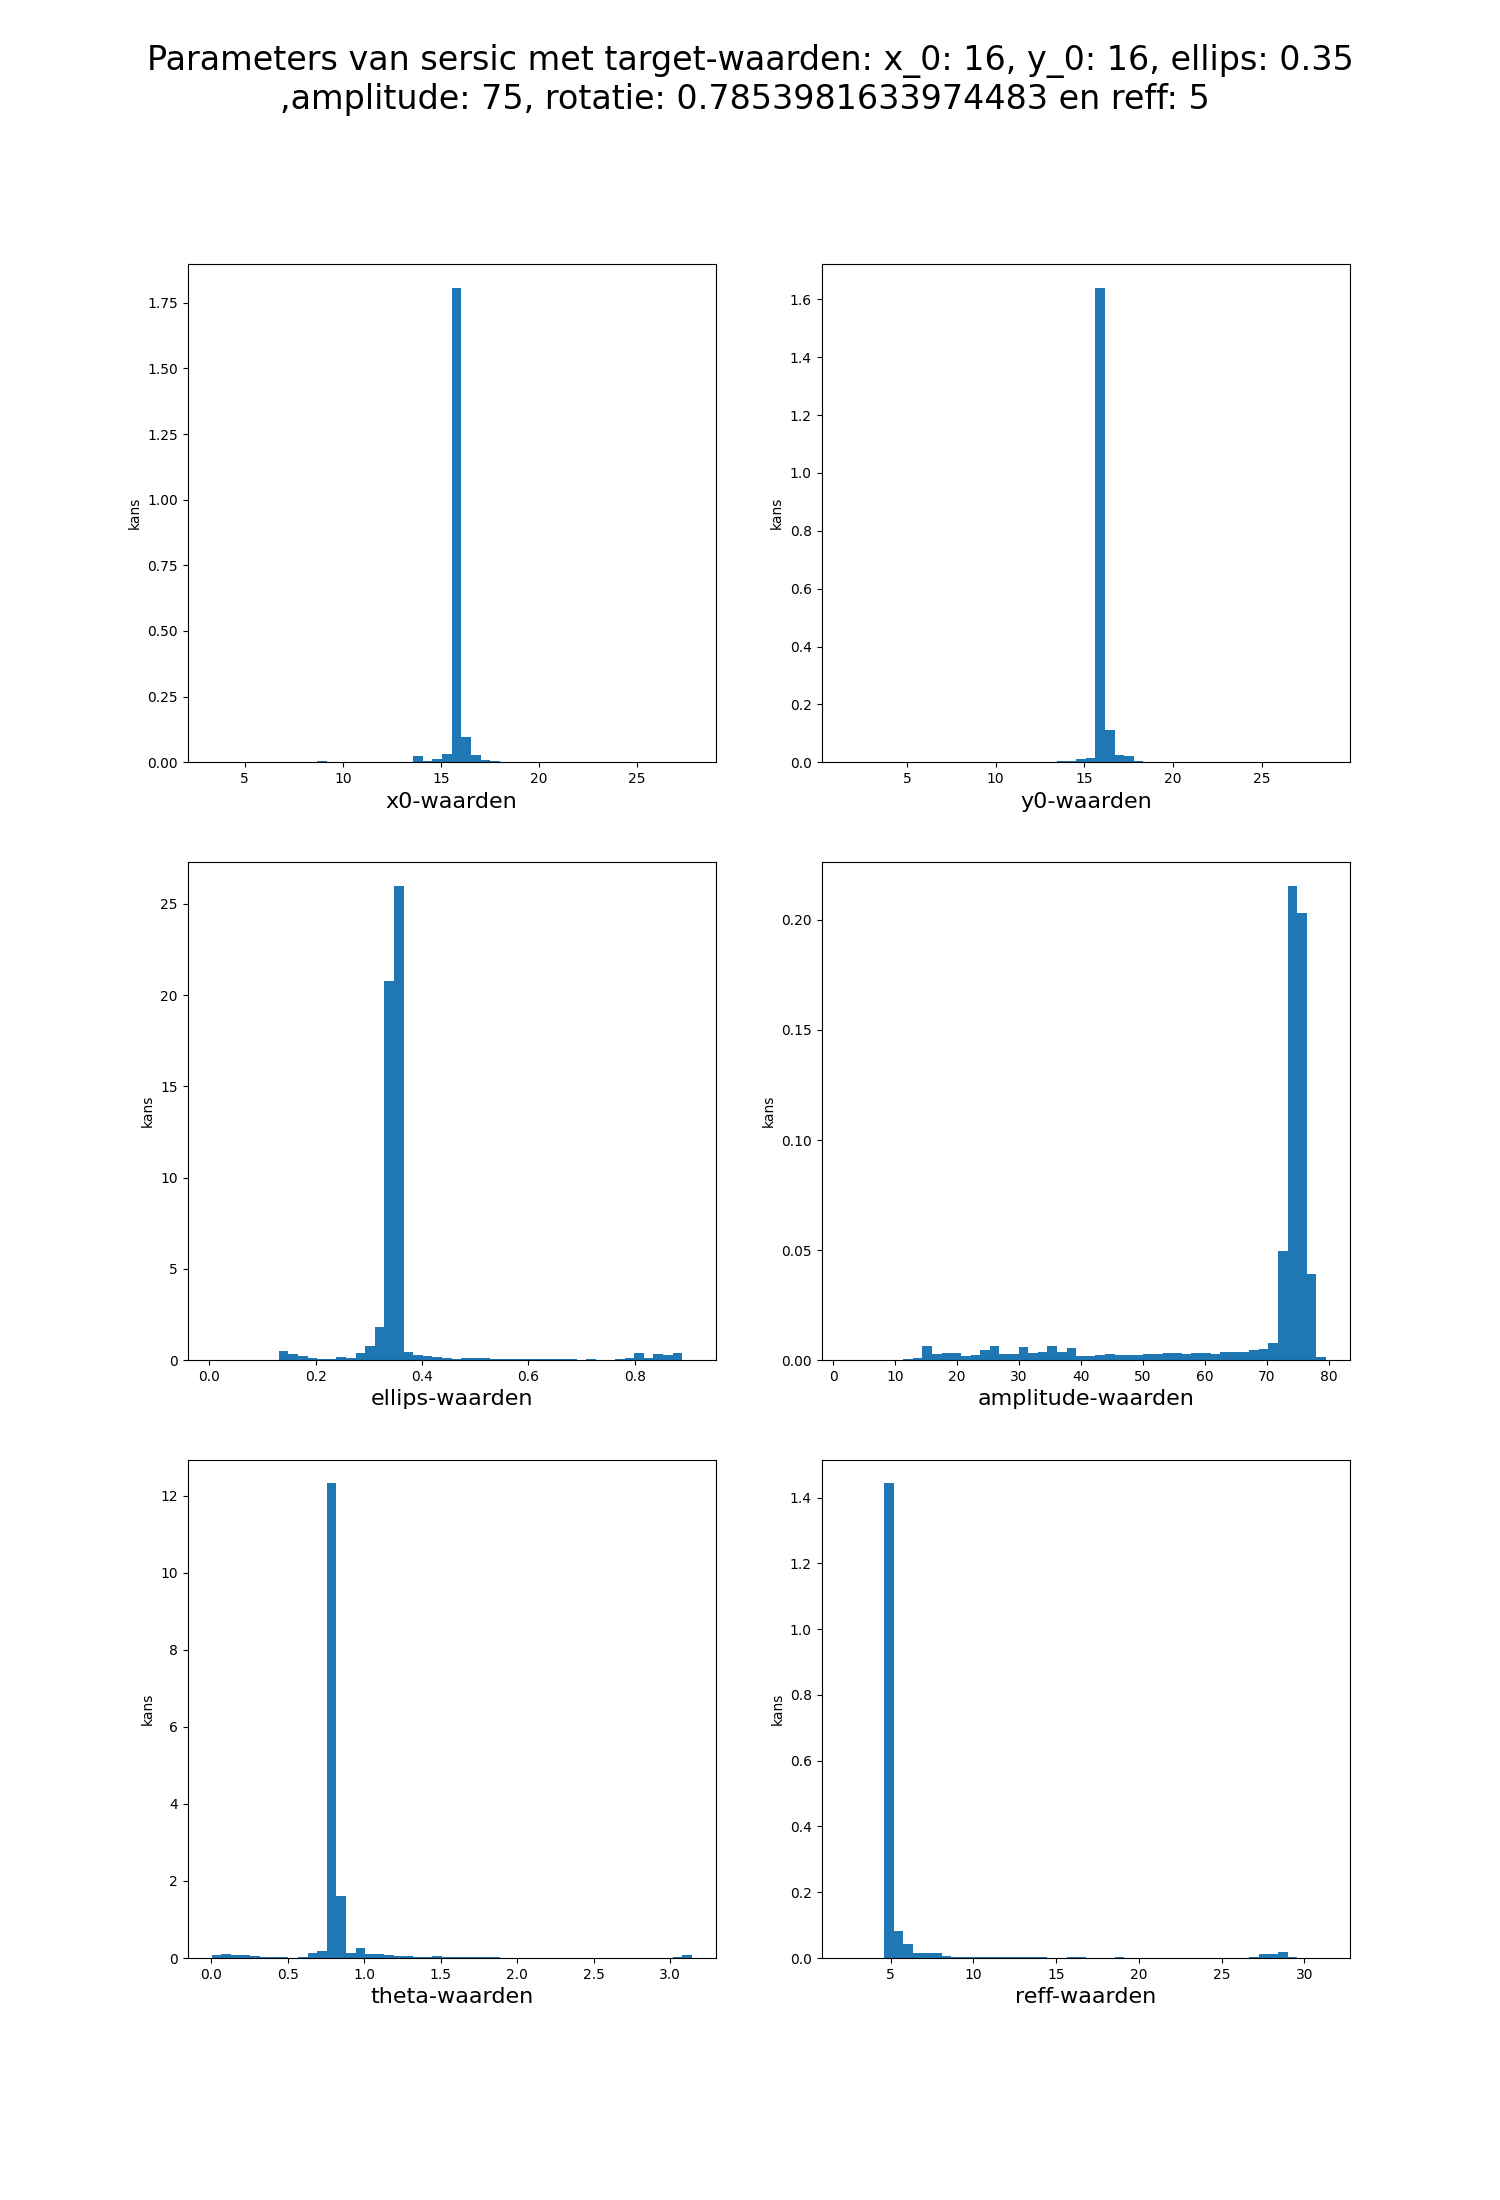
\includegraphics[width=0.95\linewidth]{Figures/emcee_hist_1200_230.png}
    \caption{Het resultaat van het afschatten van de zes parameters van de sersic, gebruikmakend van de emceee library.}
    \label{fig: emcee}
\end{figure}\mbox{}\\
Opnieuw valt het op dat de afschatting hier beter is dan met het Metropolis algoritme, doordat er een gemiddelde genomen wordt over de parameters. 

\subsection{Het afschatten van parameters van twee 2D sersic systemen}
Nu de parameters van één object afgeschat kunnen worden is het doel om ook de parameters van twee (of zelfs meerdere) objecten af te kunnen schatten. De werkwijze is volledig analoog aan het geval met slechts één object. Er wordt opnieuw gebruik gemaakt van zowel het Metropolis algoritme als de emcee library. \\ \\
Soms kan een object dat achter aan ander object staat niet waargenomen worden. Daarom is het nodig om de parameters van meerder objecten goed te kunnen schatten. Dat wordt weergegeven in \cref{fig:2_sersic}. Daar staat op de eerste foto telkens het voorgrondobject, op de tweede foto staat het achtergrondobject en op de derde foto zijn de beelden samengevoegd tot één afbeelding. Daar wordt  gezien dat het achtergrondobject soms volledig verdwijnt achter het voorgrondobject.
\begin{figure}
    \begin{minipage}{0.98\linewidth}
    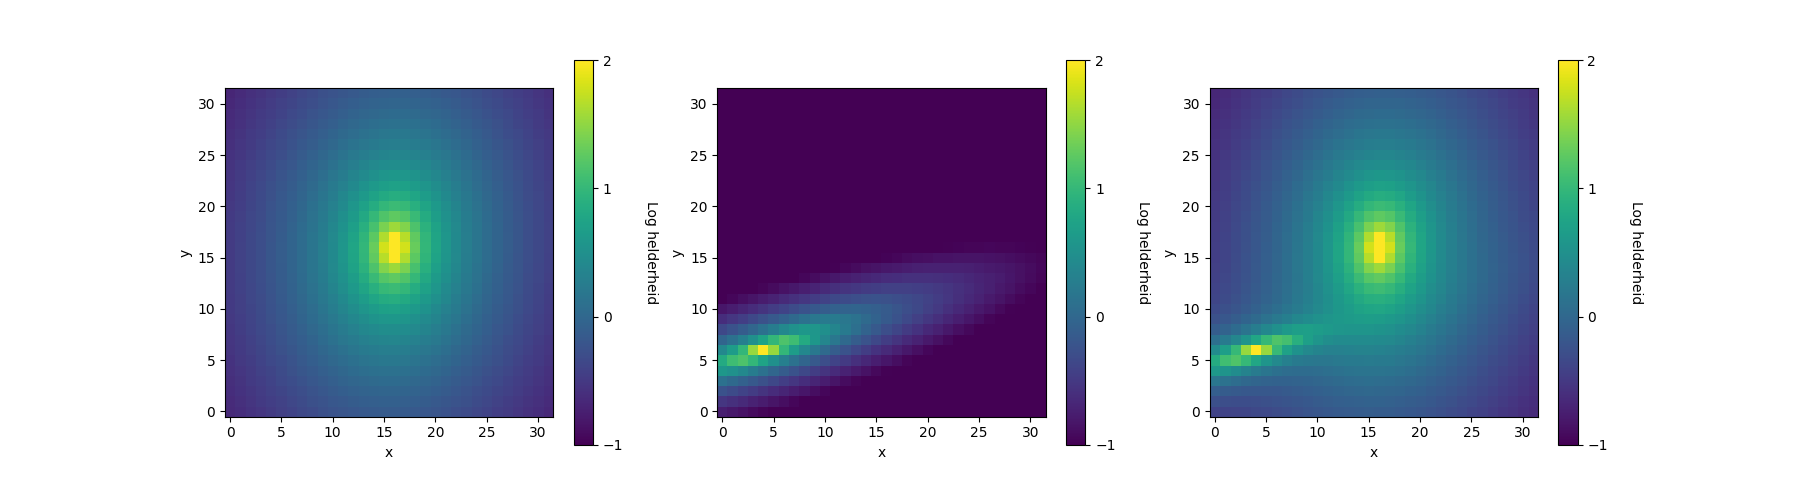
\includegraphics[width=0.95\linewidth]{Sections/figuur_2D_zonder_package_3_8_8_0.3_1.5.png}
    \subcaption{Het achtergrondobject verdwijnt helemaal achter het voorgrondobject}
    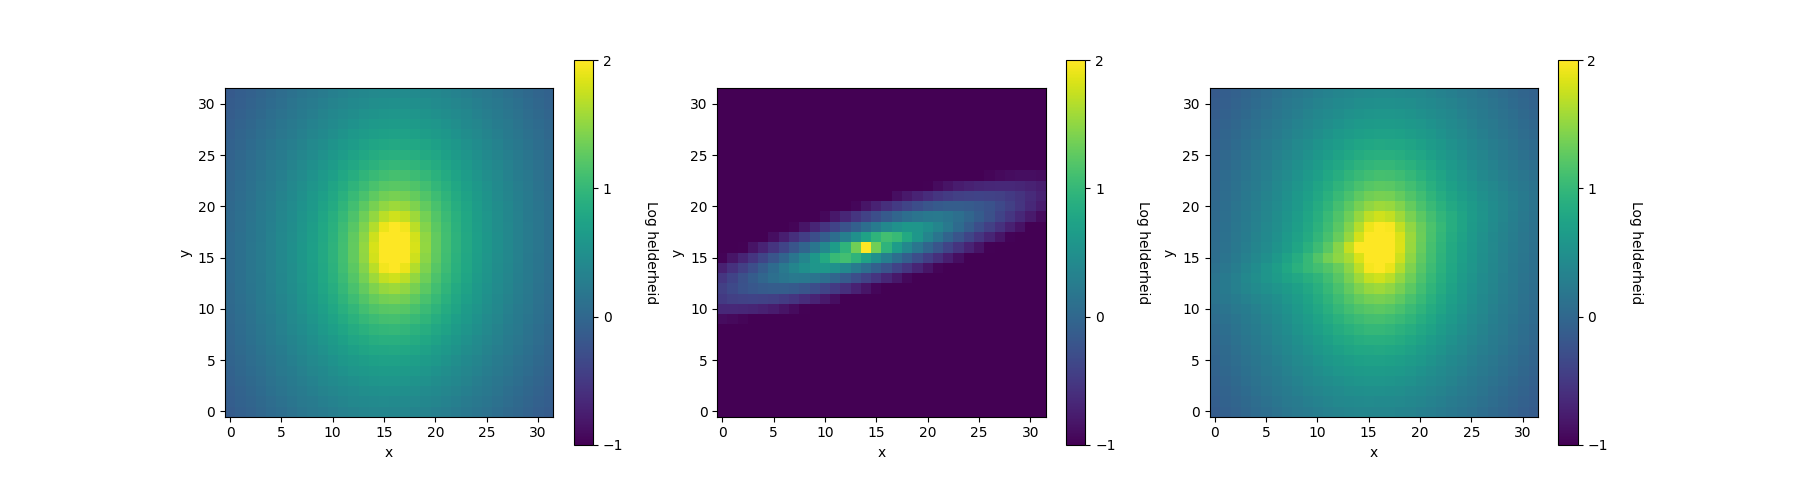
\includegraphics[width=0.95\linewidth]{Sections/figuur_2D_zonder_package_10_8_8_0.3_1.5.png}
    \subcaption{Het achtergrondobject blijft grotendeels zichtbaar na het optellen bij het voorgrondobject}
    \end{minipage}
    \caption{Op de meest linkse figuur staat het heldere voorgrondobject, op de middelste figuur staat het achtergrondobject. Op de meest rechtse figuur zie je het resultaat van het optellen van het voorgrondobject en het achtergrondobject.}
    \label{fig:2_sersic}
\end{figure}
Er werd een eerste poging gedaan tot het afschatten van de parameters van de twee sersic profielen. De resultaten ervan zijn te zien in \cref{fig: 2 sersic}. Wat opvalt is dat er op beide figuren twee pieken staan. Dat is logisch, doordat er ontaarding is. Het algoritme kan niet bepalen welke sersic nummer 1 is, en welke sersic nummer 2 is. De afgeschatte waarden komen overeen met wat er verwacht wordt, maar het is nu nog zaak om de juiste parameters te koppelen aan de juiste sersic.
\begin{figure}
    \begin{minipage}{0.98\linewidth}
    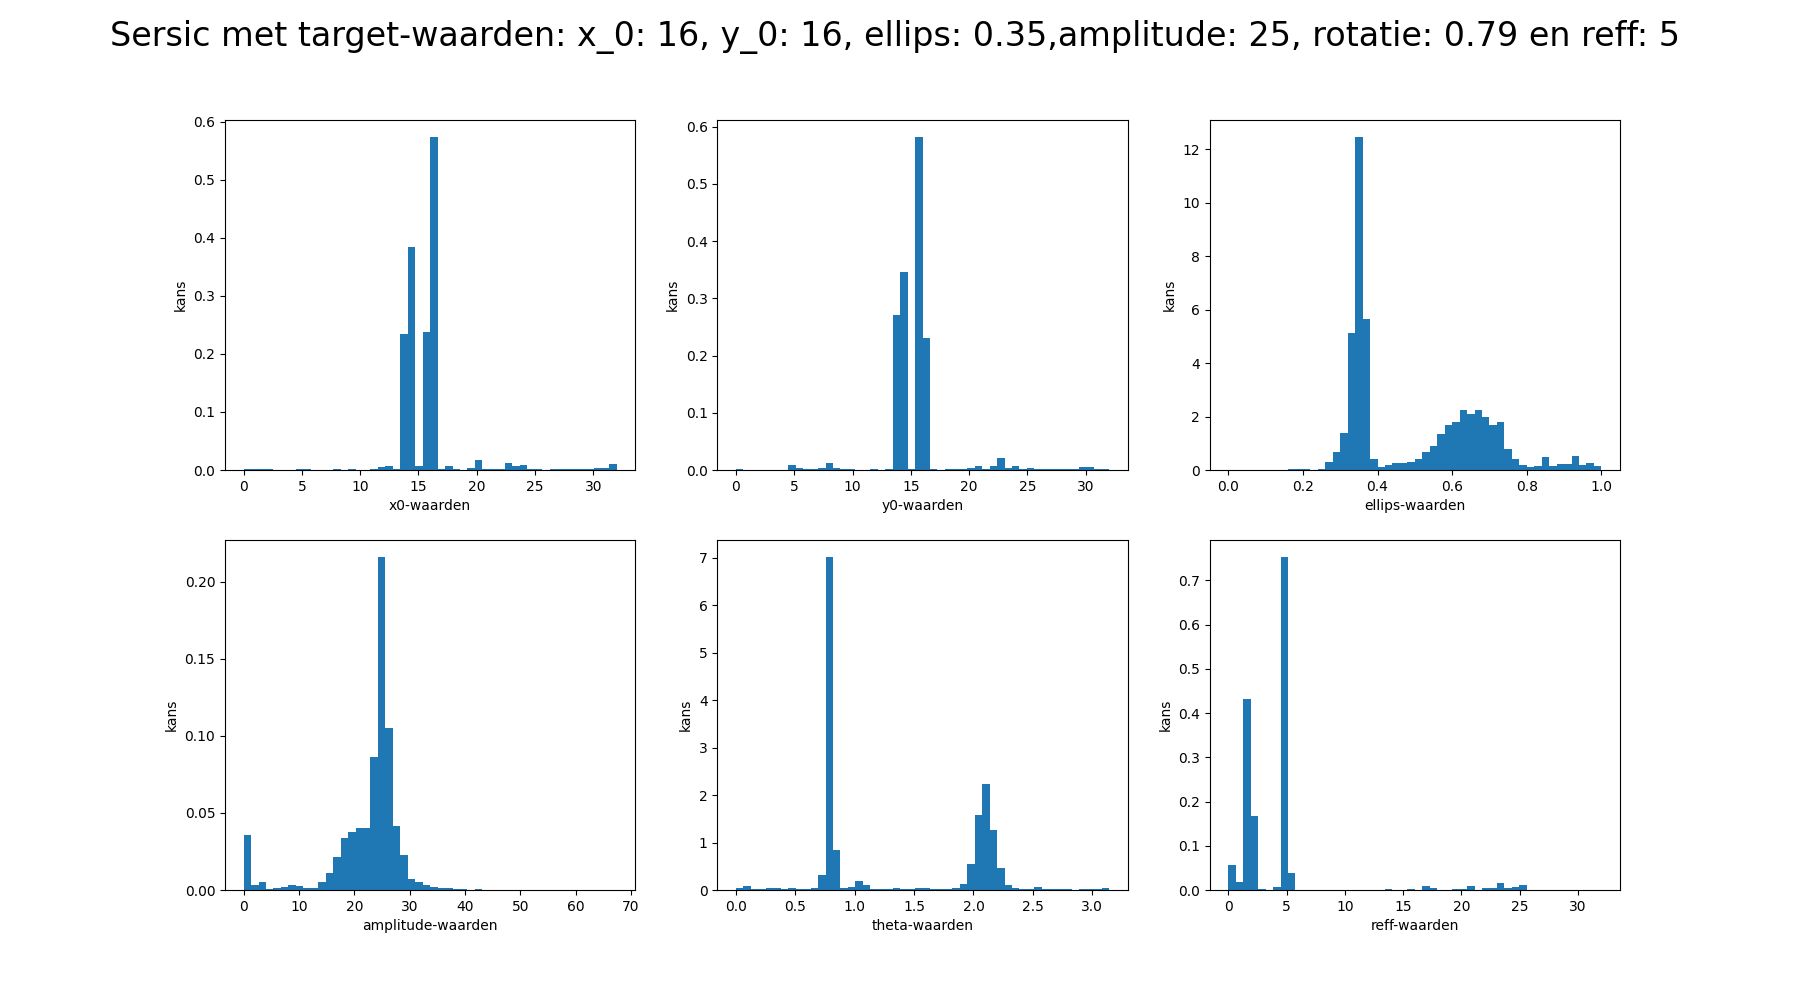
\includegraphics[width=0.95\linewidth]{Figures/1_emcee_hist_1200000_400000 (1).png}
    \subcaption{De parameters van de eerste sersic}
    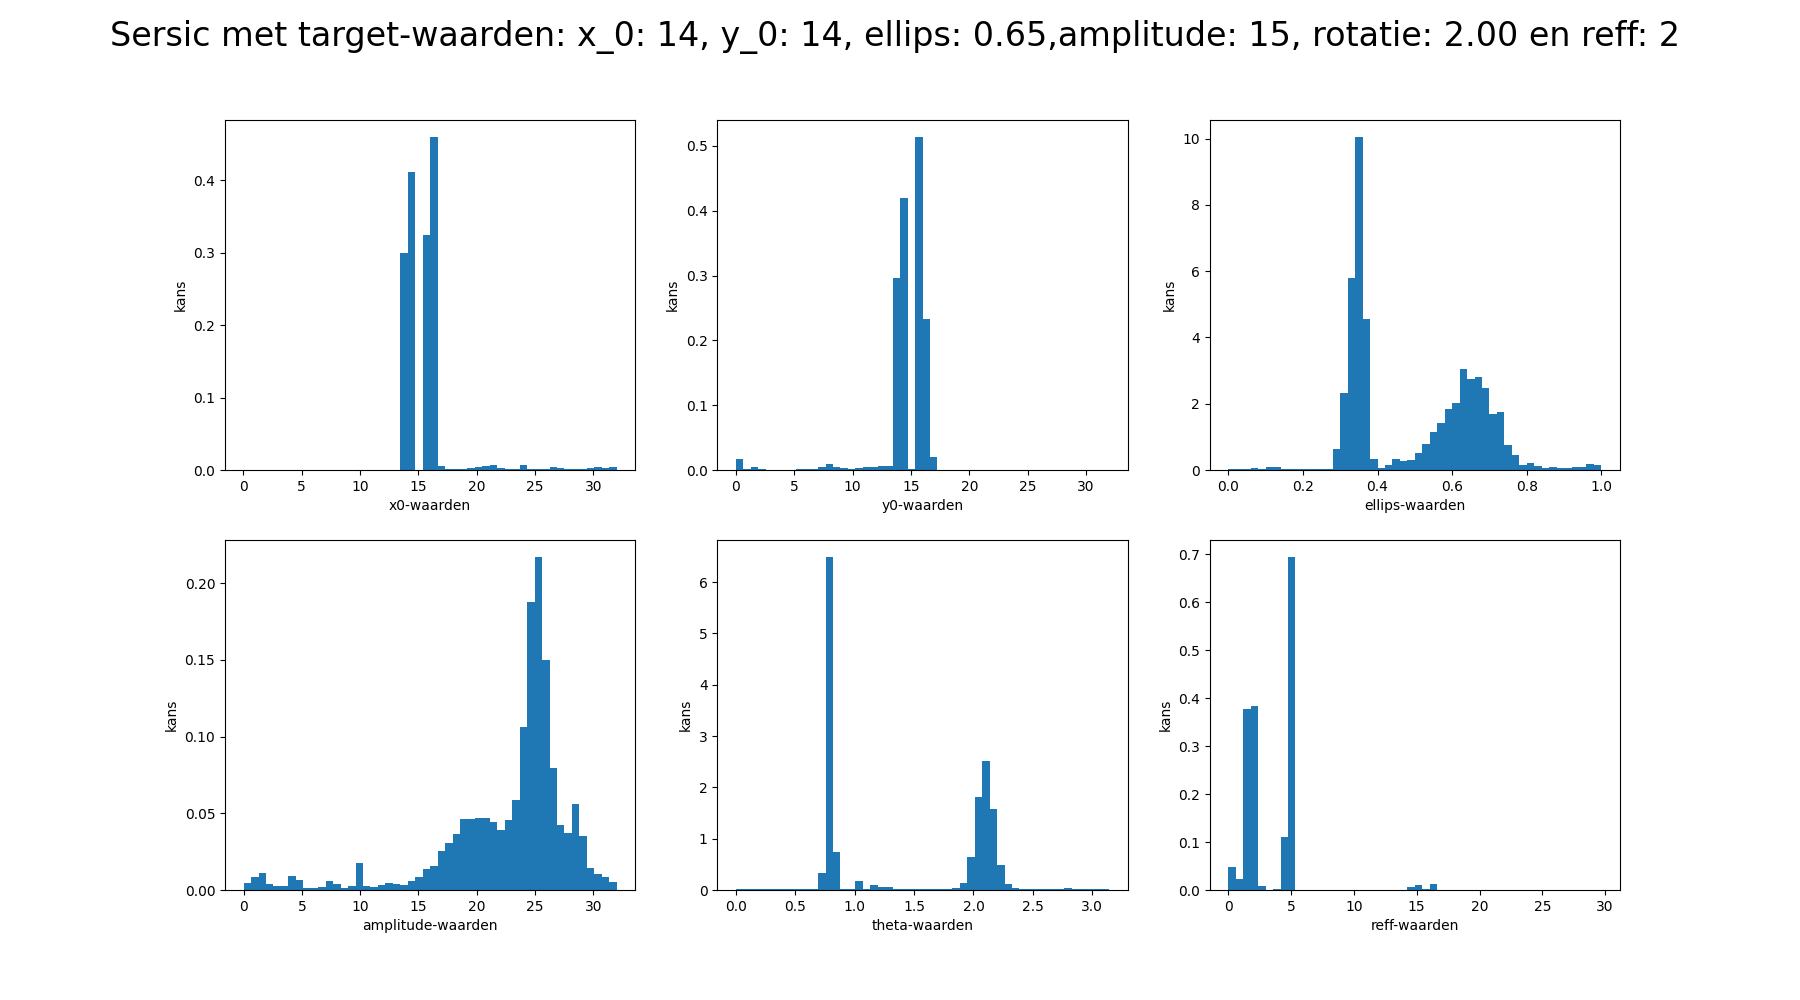
\includegraphics[width=0.95\linewidth]{Figures/2_emcee_hist_1200000_400000 (1).png}
    \subcaption{De parameters van de tweede sersic}
    \end{minipage}
    \caption{De afgeschatten parameters van een systeem waarbij twee sersics in elkaars buurt staan. De parameters van beide sersics worden afgeschat. De afgesachteen waarden komen overeen met de target waarden, maar er is nog een probleem met de ontaarding.}
    \label{fig: 2 sersic}
\end{figure}
In het proces van het genereren van de samples wordt er steeds een voorstel gedaan, een kans bepaald, en dan wordt een staat geaccepteerd of verworpen. Er wordt vanaf nu bijgehouden welke combinatie van parameters de hoogste kans had. Dan is nog niet geweten welke set van parameters sersic 1 beschrijft, en welke set van parameters sersic 2 beschrijft, maar dat hoeft geen probleem te zijn. De juiste combinaties van de parameters is dan wel gekend. Voor zowel het geval waar het achtergrondobject nog zichtbaar is, als voor het geval waar het achtergrondobject volledig achter de zware massa staat, is dit gedaan. Het resultaat is te zien in \cref{fig: 2 sersic niet ontaard} en \cref{fig: 2 sersic naast zwaar}.
\begin{figure}
    \begin{minipage}{0.98\linewidth}
        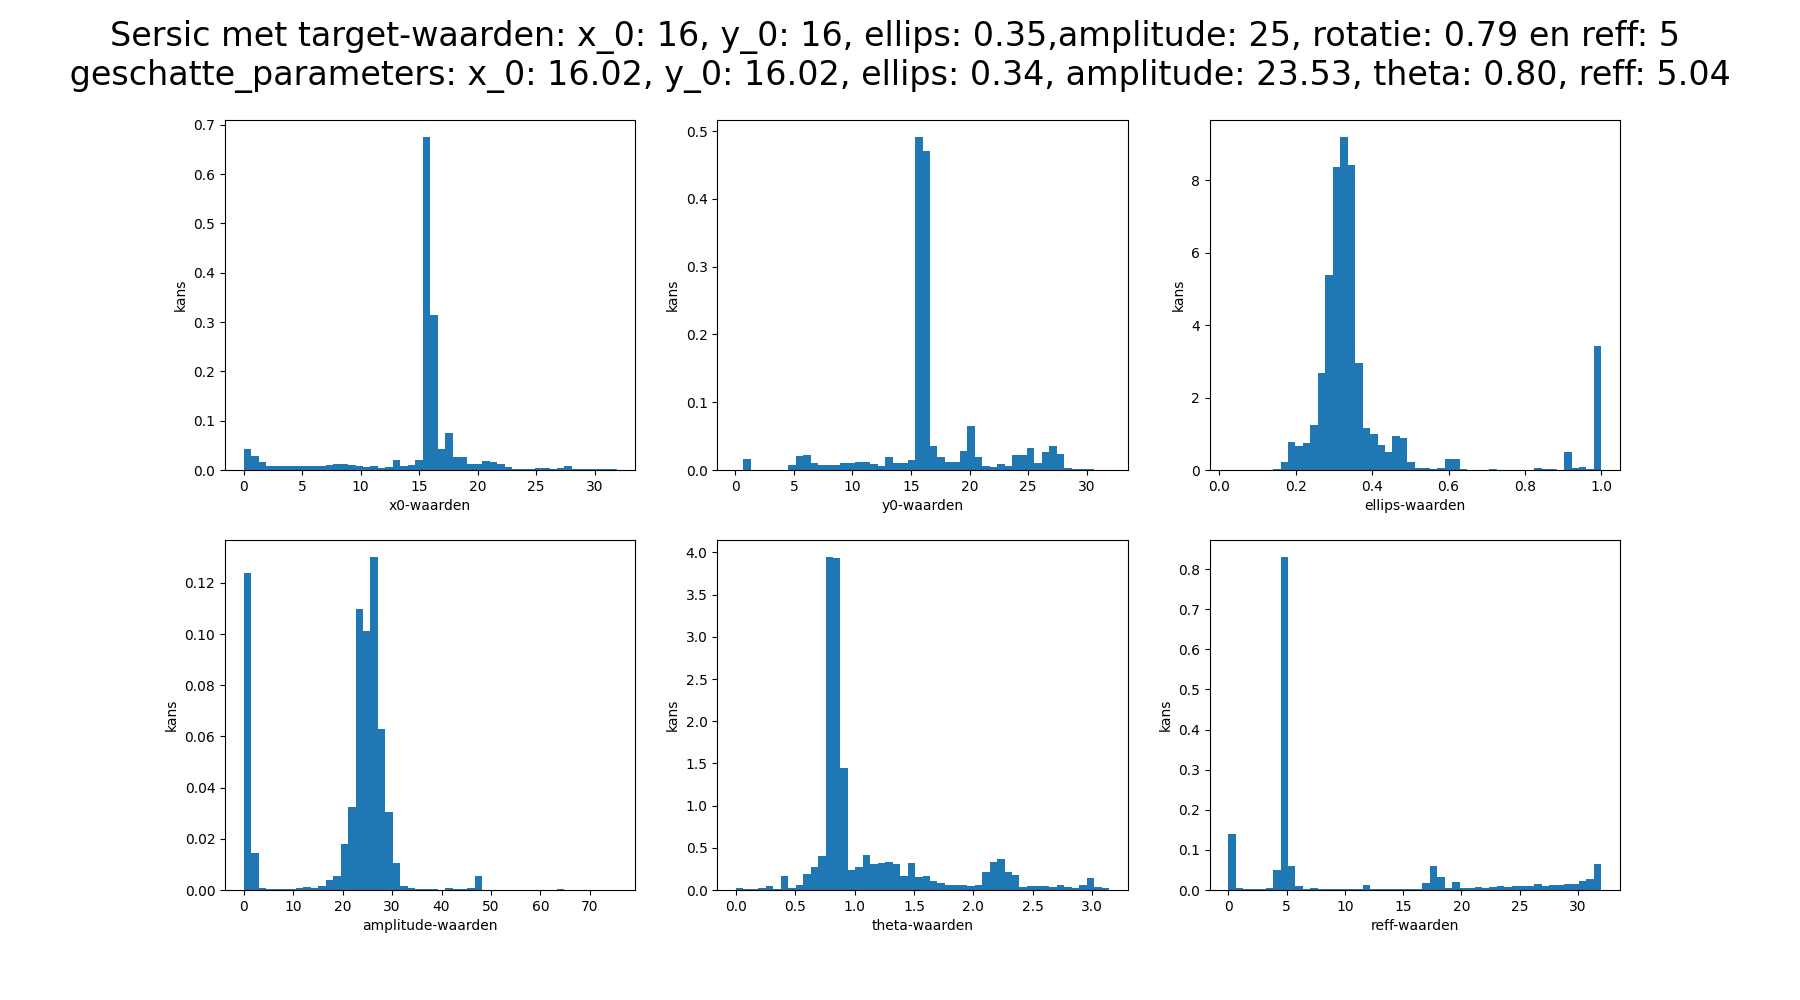
\includegraphics[width=0.95\linewidth]{Figures/1_emcee_hist_6000_750.png}   
        \subcaption{De parameters van de eerste van twee sersics}
        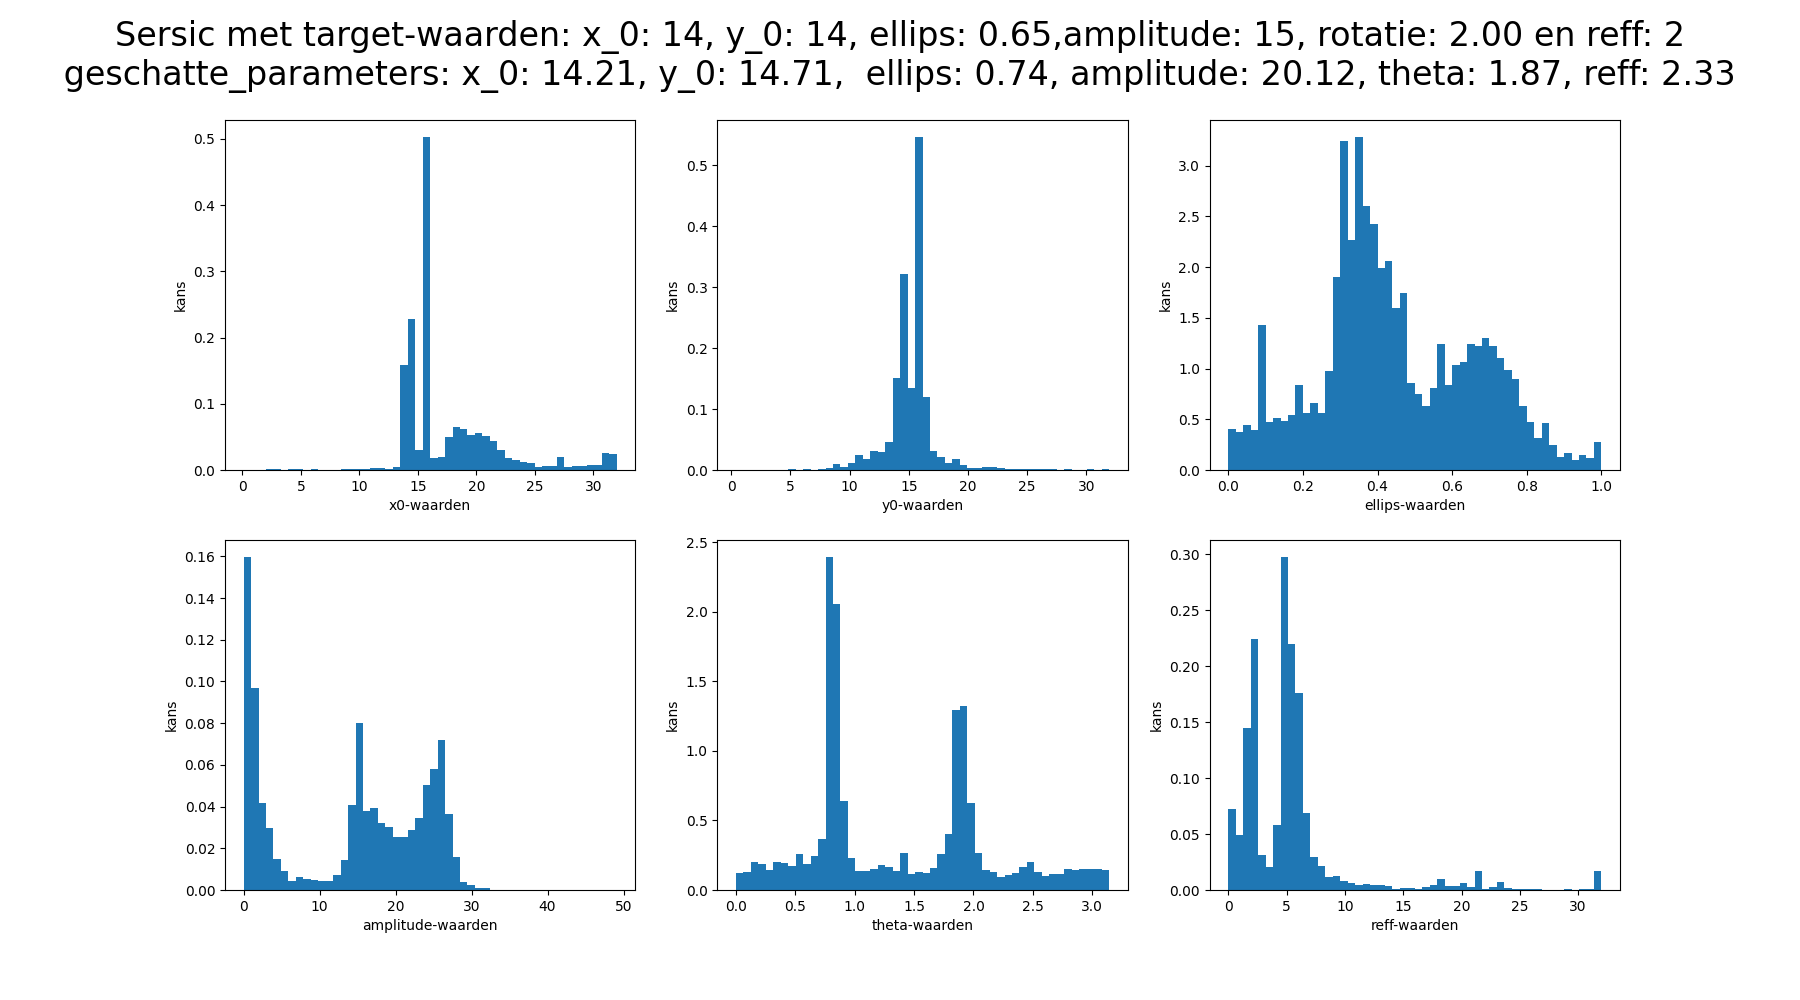
\includegraphics[width=0.95\linewidth]{Figures/2_emcee_hist_6000_750.png}
        \subcaption{De parameters van de tweede sersic}
        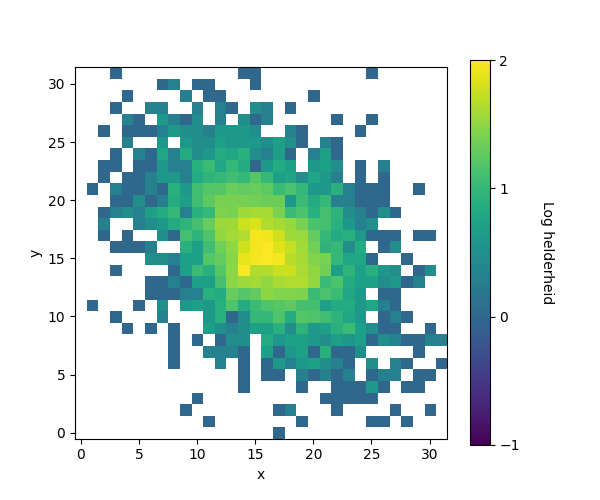
\includegraphics[width=0.95\linewidth]{Figures/figuur_2D_zonder_package_25_5_1_0.35_0.7853981633974483_6000.png}
        \subcaption{Een plot van de sersic volgens de gegenereerde data. In het midden staat duidelijk het eerste, zware, beeld. Het achtergrondbeeld is niet zichtbaar en staat achter de zware massa.}
    \end{minipage}
    \caption{De afschatting van de parameters in het geval van twee sersic (waarbij de ene sersic achter de andere staat) in dezelfde figuur. Naast de parameters wordt ook steeds de plot van de af te schatten sersic gegenereerd. Op de grafieken is nog steeds ontaarding te zien, maar het koppelen van de juiste parameters lukt door gebruik te maken van onze methode van de grootste kans}
    \label{fig: 2 sersic niet ontaard}
\end{figure}
\begin{figure}
    \begin{minipage}{0.98\linewidth}
        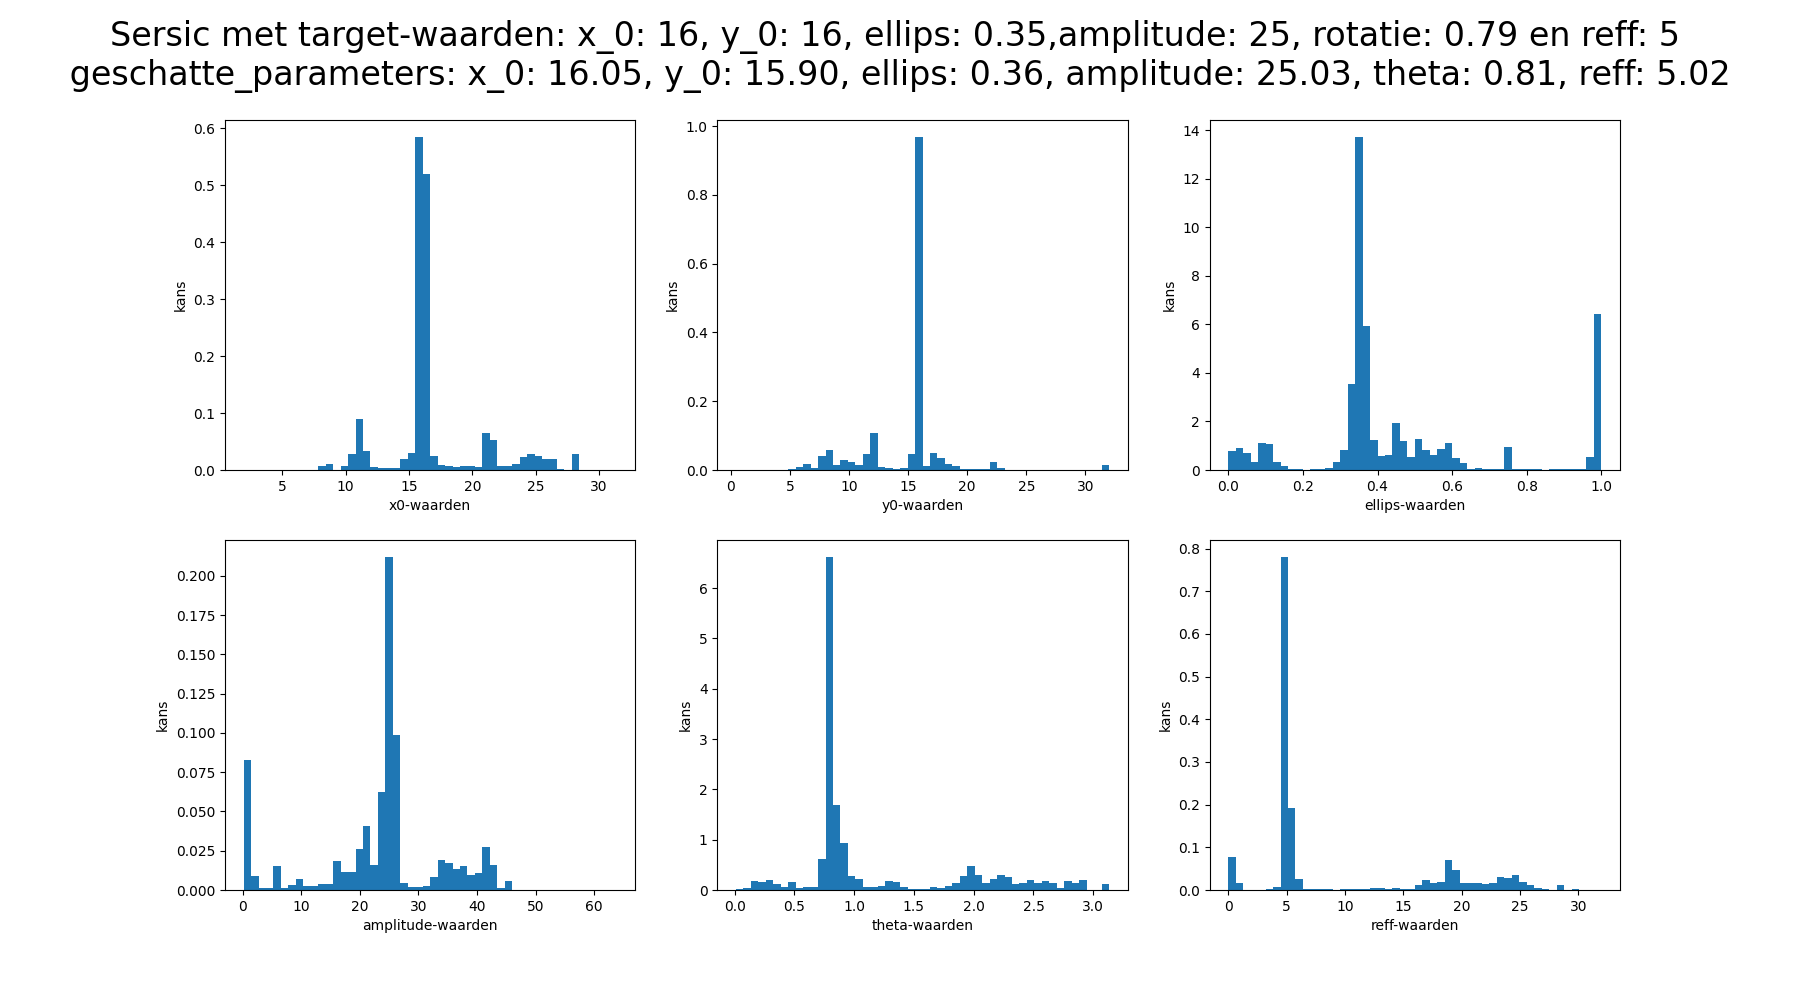
\includegraphics[width=0.95\linewidth]{Figures/1_emcee_hist_5000_750.png}   
        \subcaption{De parameters van de eerste van twee sersics}
        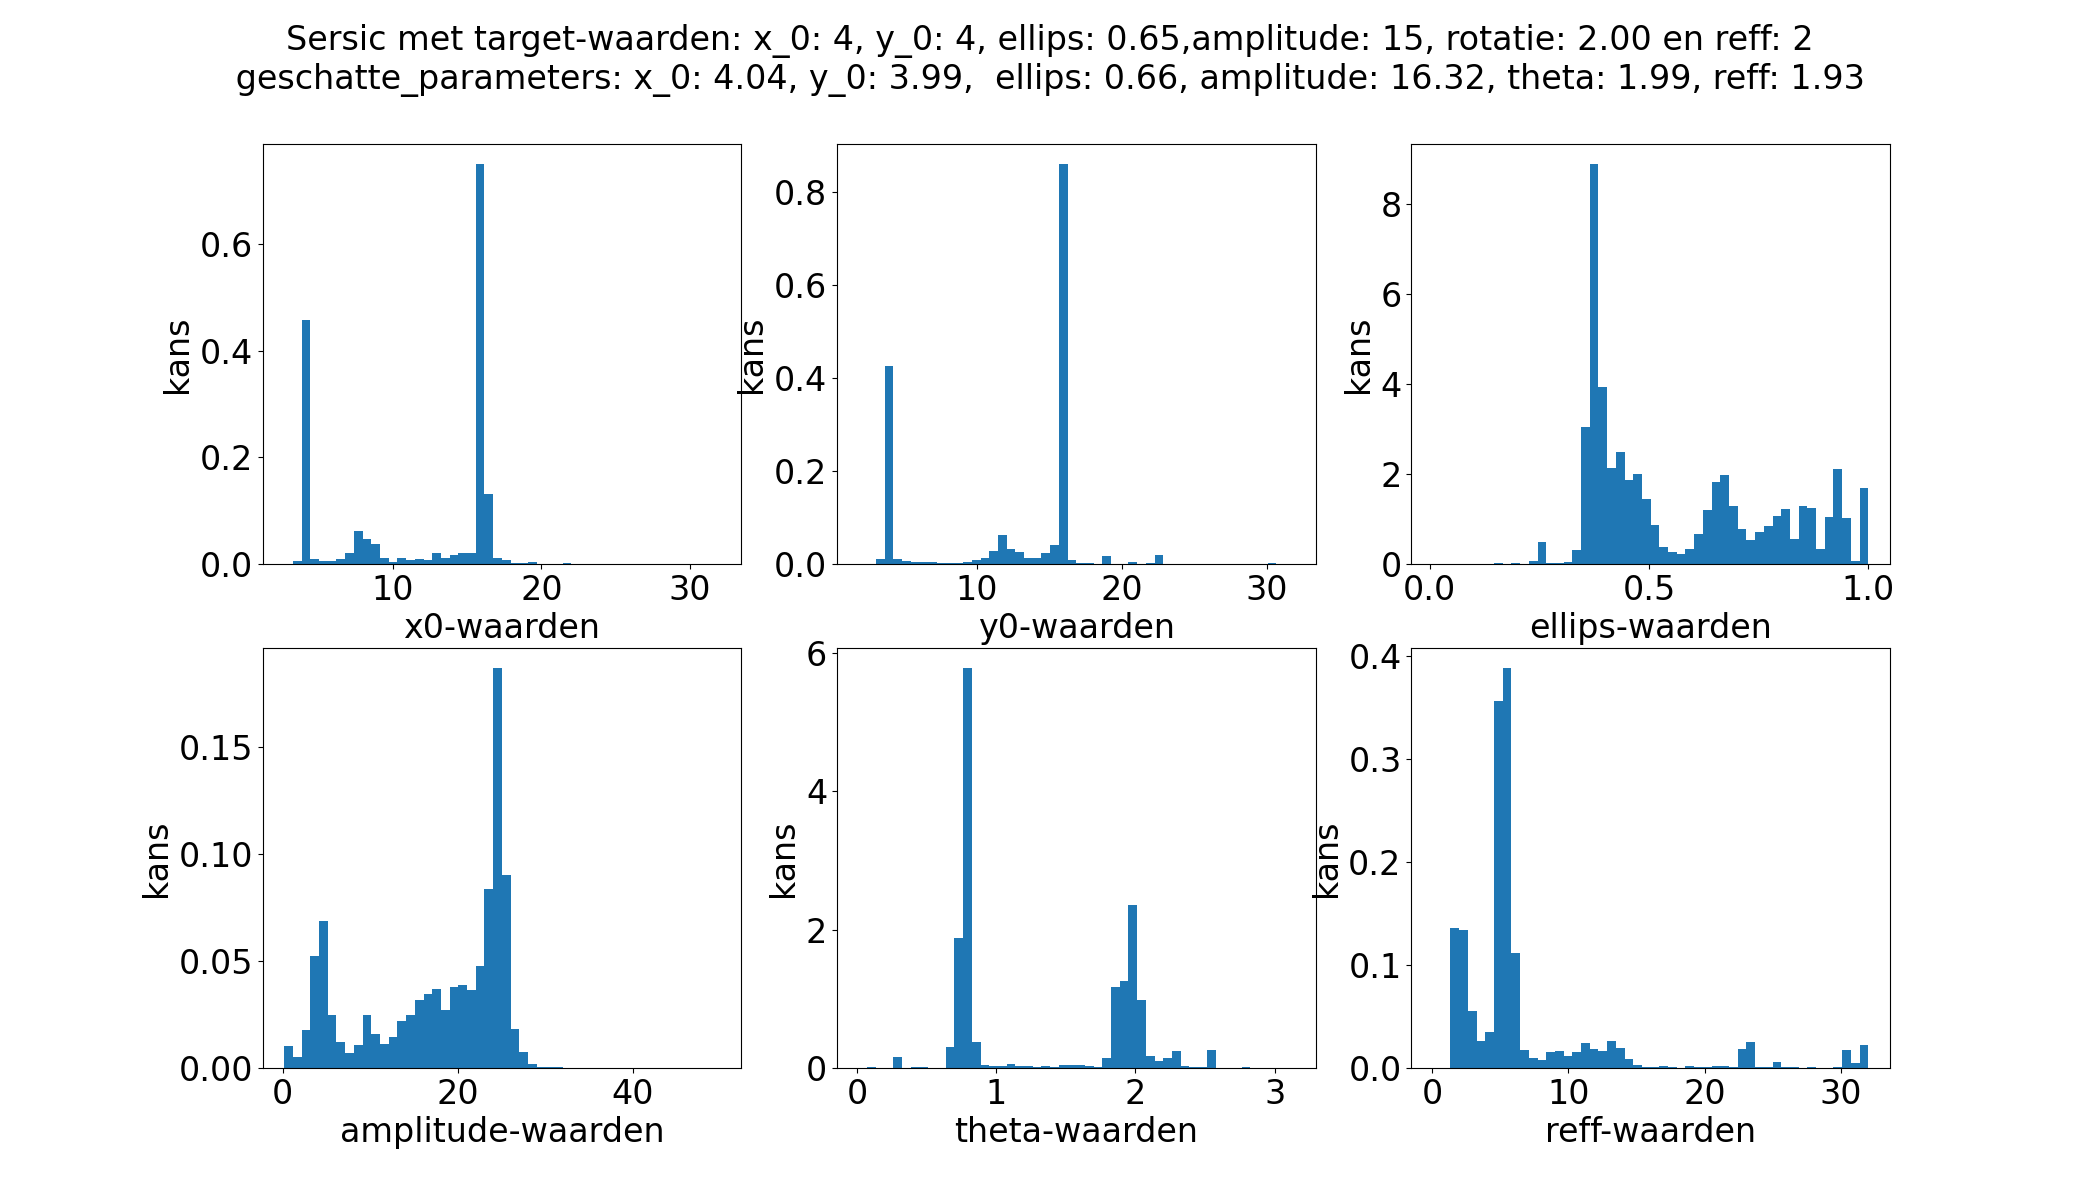
\includegraphics[width=0.95\linewidth]{Figures/2_emcee_hist_5000_750.png}
        \subcaption{De parameters van de tweede sersic}
        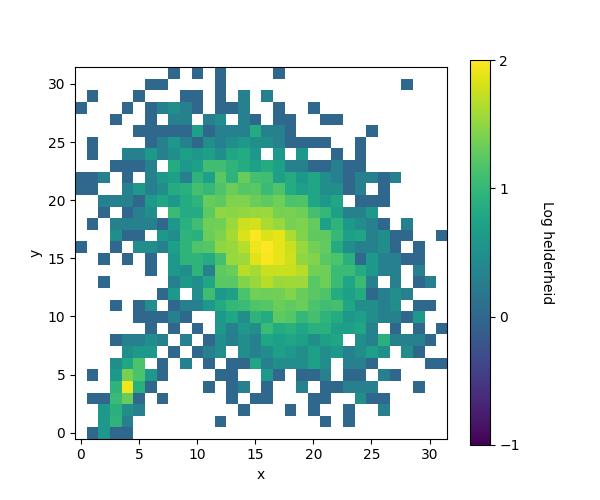
\includegraphics[width=0.95\linewidth]{Figures/figuur_2D_zonder_package_25_5_1_0.35_0.7853981633974483_5000.png}
        \subcaption{Een plot van de sersic volgens de gegenereerde data. We zien duidelijk dat het kleine beeldje langs de zware massa staat.}
    \end{minipage}
    \caption{De afschatting van de parameters in het geval van twee sersic (die naast elkaar staan) in dezelfde figuur. Naast de parameters wordt ook steeds de plot van de af te schatten sersic gegenereerd. Op de figuren is nog steeds ontaarding te zien, maar het koppelen van de juiste parameters lukt door gebruik te maken van onze methode van de grootste kans}
    \label{fig: 2 sersic naast zwaar}
\end{figure}
In beide gevallen kunnen de parameters van beide sersics goed afgeschat worden. Op deze manier kan het beeld dat achter de zware massa staat gereconstrueerd worden.

\subsection{De afschatting van parameters van een 2D sersic systeem met een werkelijke achtergrond}
In de voorgaande bepaling van de parameters van het sersic profiel werden aan de dataset van de werkelijke waarden wat ruis toegevoegd. Nu wordt overgegaan op een meer werkelijke toestand door een achtergrond te voorzien die gemodelleerd is door NASA. De achtergrond die gebruikt wordt is te zien in \cref{fig:NASA}.
\begin{figure}
    \begin{minipage}{0.98\linewidth}
        \centering
       \includegraphics[width=0.55\linewidth]{Figures/achtergrond_groot.jpg}
        \subcaption{Een achtergrondbeeld gemodelleerd door NASA. Foto van \cite{nasa-2023}}
        \label{fig:NASA} 
        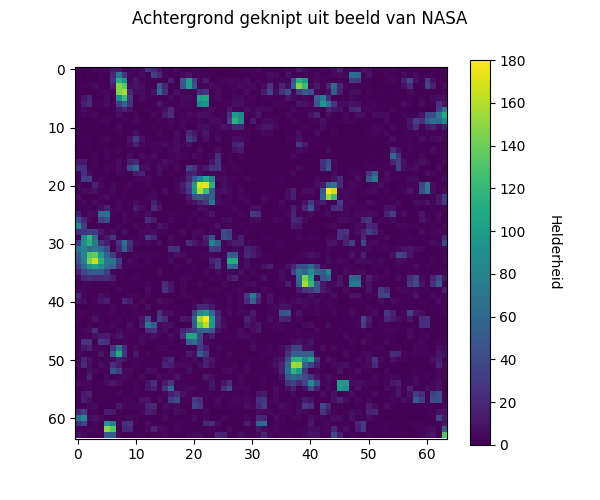
\includegraphics[width=0.85\linewidth]{Figures/sersic_achtergrond.png}
        \subcaption{Figuur van grootte 64x64 bekomen uit het achtergrondbeeld gegenereerd door NASA, \cref{fig:NASA}.}
        \label{fig: kleine achtergrond}
        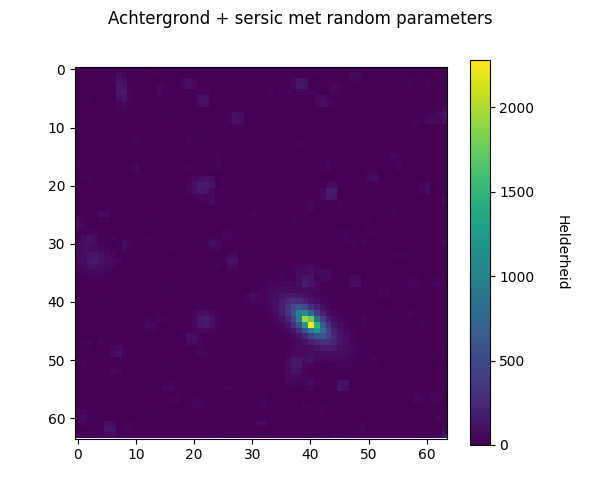
\includegraphics[width=0.85\linewidth]{Figures/sersic+achtergrond.png}
        \caption{Een 2D sersic profiel op een werkelijke achtergrond.}
        \label{fig:achtergrond+sersic}
    \end{minipage}
    \caption{De opbouw van het genereren van een sersic op een werkelijke achtergrond. Eerst wordt een deeltje geknipt uit de werkelijke achtergrond, er wordt een sersic gegeneerd met willekeurige paramters. De sersic wordt opgeteld bij de achtergrond en geeft zo een ruisig geheel dat de werkelijkheid weerspiegeld.}
\end{figure}
Dit is een zeer grote foto, voor de achtergrond in het programma werd een deeltje van 64x64 genomen uit deze afbeelding. Zo'n figuur is te zien in \cref{fig: kleine achtergrond}.
Hierop werd dan een sersic geplaatst om zo tot een nieuw ruizig geheel te komen. Zo'n sersic op de werkelijke achtergrond is te zien in \cref{fig:achtergrond+sersic}.
\\
Het uiteindelijke doel is nu om de waarden van de sersic af te schatten om zo enkel de achtergrond te bekomen. De afschatting van de parameters van deze sersic wordt gedaan door gebruik te maken van de emcee library.
\\ \\
In het begin werd het programma geholpen en werden alle af te schatten parameters als gekend beschouwd. Zo kon de oorspronkelijke sersic exact nagemaakt worden. Deze gegenereerde sersic is te zien in \cref{fig: gegenereerde sersic}. 
\begin{figure}
    \begin{minipage}{0.98\linewidth}
        \centering
        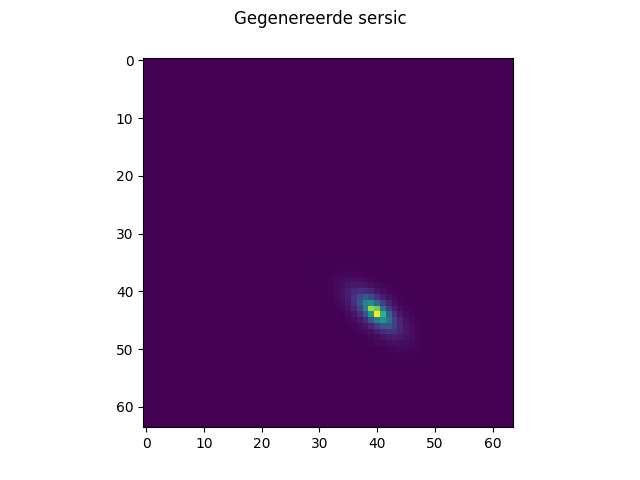
\includegraphics[width=0.95\linewidth]{Figures/gegenereerde_sersic.png}
        \subcaption{Een sersic gemodelleerd uit de afgeschatte parameters van de totale figuur, \cref{fig:achtergrond+sersic}.}
        \label{fig: gegenereerde sersic}
        \centering
        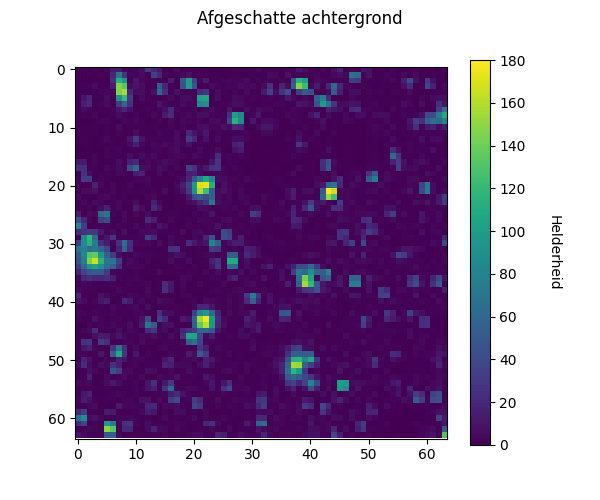
\includegraphics[width=0.85\linewidth]{Figures/afgeschatte_achtergrond.png}
        \subcaption{De afgeschatte achtergrond.}
        \label{fig:afgeschatte achtergrond}
    \end{minipage}
    \caption{Het proces van het afschatten van de achtergrond wordt weergegeven. Er wordt vertrokken vanuit de ruizige sersic (\cref{fig:achtergrond+sersic}). Dan worden de paramters van die ruizige sersic afgeschat. Met de methode van de grootste kans wordt zo een sersic getekend, die is te zien in \cref{fig: gegenereerde sersic}. Om de achtergrond te bekomen wordt de sersic afgetrokken van het ruizig geheel, wat resulteerd in de oorspronkelijke achtergrond (\cref{fig:afgeschatte achtergrond}).}
\end{figure}
De gegenereerde sersic (\cref{fig: gegenereerde sersic}) wordt afgetrokken van het totaal (\cref{fig:achtergrond+sersic}). Op die manier wordt de achtergrond gevonden. De afgeschatte achtergrond is te zien in \cref{fig:afgeschatte achtergrond}. 

Er wordt nu opgemerkt dat de afgeschatte achtergrond en de oorspronkelijke achtergrond genomen uit het beeld van NASA exact overeenkomen.\\ \\
Nu wordt exact hetzelfde gedaan, maar worden de zes parameters allemaal afgeschat. Op een analoge manier wordt de achtergrond afgeschat. De achtergrond geknipt uit het beeld van NASA is te zien in \cref{fig:achtergrond nasa} en de afgeschatte achtergrond is te zien in \cref{fig:geschatte achtergrond}.
\\ \\
\begin{figure}
    \begin{minipage}{0.98\linewidth}
        \centering
        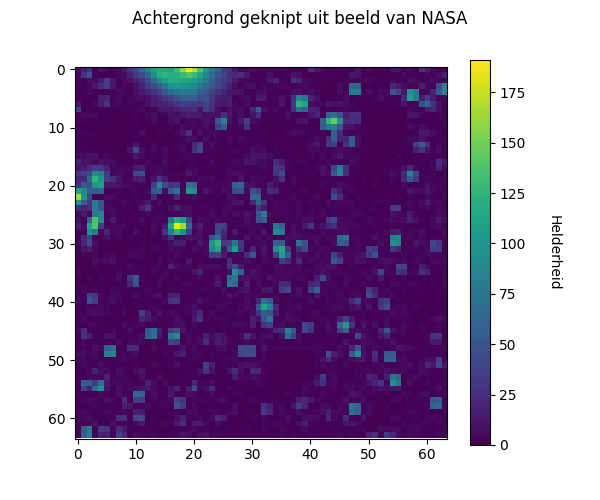
\includegraphics[width=0.95\linewidth]{Figures/sersic_achtergrond2.png}
        \subcaption{De achtergrond geknipt uit de gemodelleerde achtergrond van NASA}
        \label{fig:achtergrond nasa}
        \centering
        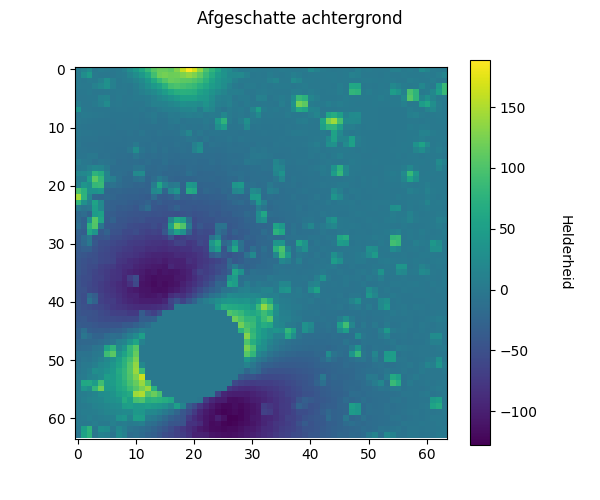
\includegraphics[width=0.95\linewidth]{Figures/afgeschatte_achtergrond2.png}
        \subcaption{De afgeschatte achtergrond, waarin de zes parameters van de sersic afgeschat werden.}
        \label{fig:geschatte achtergrond}
    \end{minipage}
    \caption{De vergelijking tussen de oorspronkelijke achtergrond (\cref{fig:achtergrond nasa}) de afgeschatte achtergrond (\cref{fig:geschatte achtergrond}). Over het algemeen komen de figuren goed overeen, maar op de afgeschatte achtergrond is wel duidelijk te zien dat sersic niet volledig correct afgeschat is.}
\end{figure}

Op de figuren is te zien dat de afgeschatte achtergrond wel goed overeenkomt met de werkelijke achtergrond. Wat wel opvalt is dat de parameters van de sersic niet zo goed afgeschat zijn. Daardoor blijft een deel van de sersic zichtbaar en zijn we nog niet in staat om de objecten achter de sersic te zien. 











\input{Sections/5-DISCUSSION}
\section{CONCLUSION}
% Edit below
Er kan geconcludeerd worden dat zowel de stelling van Bayes, het Metropolis algoritme en de emcee library leiden tot goede resultaten. De parameters van een sersicsysteem bestaande uit één sersic konden afgeschat worden. Ook de paramters van een systeem met twee sersics konden afgeschat worden. Op die manier kan er info bekomen worden van het beeld achter de zware massa. Ook werd er geprobeerd om van een sersic op een werkelijke achtergrond de parameters van de sersic af te schatten om zo de achtergrond te reconstrueren. Dit zou gebruikt kunnen worden om een AI te trainen, die dan zelf de sersic van de achtergrond zou kunnen halen om de achtergrond zelf te reconstrueren. \\ \\
Het afschatten van de waarden van de sersic op de werkelijke achtergrond ging niet zo goed, vermoedelijk doordat de werkelijke achtergrond veel ruiziger is dan de poissonruis die toegevoegd werd aan de sersic in de eerdere afschattingen. 

% Additional sections for acknowledgments
\rule{\linewidth}{0.4pt}
\textit{Author contributions}
% Edit below
JL heeft het onderzoek bedacht en vorm gegeven.
YR heeft de algoritmes geschreven en er experimenten mee gedaan. \\ \\
\textit{Acknowledgements} 
YR bedankt JL voor de begeleiding en ondersteuning. 
% Edit below
\newpage

% The bibliography is added at the end of the paper in a single column
\vspace{0.5cm}
\printbibliography[title={REFERENCES}]

\end{document}